\documentclass[landscape]{article}
\usepackage[a4paper,margin=3mm,landscape]{geometry}
\usepackage[scaled=0.92]{helvet}
\usepackage{multicol, multirow}
\usepackage{makecell}
\usepackage{array} 
\usepackage[table]{xcolor}
\usepackage{enumitem} 
\usepackage{amssymb}
\usepackage{graphicx}
\usepackage{amsmath}
\setlist{nosep}

\graphicspath{{./images/}}

\pdfinfo{
    /Title (CS2109S Cheatsheet.pdf)
    /Creator (TeX)
    /Producer (pdfTeX 1.40.0)
    /Author (Selwyn Ang)
    /Subject (CS2109S)
    /Keywords (CS2109S, Cheatsheet, NUS, Introduction to Artificial Intelligence and Machine Learning) 
}

% Turn off header and footer
\pagestyle{empty}


\makeatletter
\DeclareRobustCommand\smaller{\@setfontsize\smaller{6pt}{6.5pt}}
\makeatother

% redefine section commands to use less space
\makeatletter
\renewcommand{\section}{\@startsection{section}{1}{0mm}%
  {-0.1ex plus -0.1ex minus -0.1ex}%
  {0.1ex plus .1ex minus 0.1ex}%
{\normalfont\small\bfseries}}
\renewcommand{\subsection}{\@startsection{subsection}{2}{0mm}%
  {-0.1ex plus -0.1ex minus -0.1ex}%
  {0.1ex plus .1ex minus 0.1ex}%
{\normalfont\scriptsize\bfseries}}
\renewcommand{\subsubsection}{\@startsection{subsubsection}{3}{0mm}%
  {-0.1ex plus -0.1ex minus -0.1ex}%
  {0.1ex plus .1ex minus 0.1ex}%
{\normalfont\smaller\bfseries}}%
\makeatother



\renewcommand{\familydefault}{\sfdefault}
\renewcommand\rmdefault{\sfdefault}
%  makes nested numbering (e.g. 1.1.1, 1.1.2, etc)
\renewcommand{\labelenumii}{\theenumii}
\renewcommand{\theenumii}{\theenumi.\arabic{enumii}.}
\renewcommand\labelitemii{•}
\renewcommand\labelitemiii{•}

\setlength{\parindent}{0pt}
\setlength{\parskip}{0pt plus 0.5ex}
\setlength{\columnsep}{0.2cm}
%% adjust spacing for all itemize/enumerate
\setlength{\leftmargini}{0.5cm}
\setlength{\leftmarginii}{0.5cm}
\setlist[itemize,1]{leftmargin=2mm,labelindent=1mm,labelsep=1mm}
\setlist[itemize,2]{leftmargin=2mm,labelindent=1mm,labelsep=1mm}
\setlist[itemize,3]{leftmargin=2mm,labelindent=1mm,labelsep=1mm}
\setlist[enumerate,1]{leftmargin=2mm,labelindent=1mm,labelsep=1mm}
\setlist[enumerate,2]{leftmargin=2mm,labelindent=1mm,labelsep=1mm}
\setlist[enumerate,3]{leftmargin=2mm,labelindent=1mm,labelsep=1mm}

% tightcenter
\newenvironment{tightcenter}{%
  \setlength\topsep{0pt}
  \setlength\parskip{0pt}
  \begin{center}
    }{%
  \end{center}
}

% boxed
\newenvironment{tightbox}{%
  \setlength\topsep{0pt}
  \setlength\parskip{0pt}
  \begin{center}
    \begin{tabular}{|@{\hspace{\dimexpr\fboxsep+0.5\arrayrulewidth}}c@{\hspace{\dimexpr\fboxsep+0.5\arrayrulewidth}}|}
      \hline
    }
    {%
    \\ \hline
    \end{tabular}
  \end{center}
}

% fixed width box
\newenvironment{fixedbox}[1][0.7]{
  \setlength\topsep{0pt}
  \setlength\parskip{0pt}
  \begin{center}
    \begin{tabular}{|>{\centering\arraybackslash}m{#1\linewidth}|}
    \hline
  }{
  \\ \hline
  \end{tabular}
  \end{center}
}

% definition of a new term
\usepackage{soul}
\definecolor{paleyellow}{RGB}{251,243,218}
\newcommand{\definition}[2][]{\sethlcolor{paleyellow}\hl{\textbf{#2}} #1  $\rightarrow$}
% inline definition
\newcommand{\ildefinition}[1]{\sethlcolor{paleyellow}\hl{\textbf{#1}}}

% important note (attention)
\newcommand{\attention}{{\color{red}\textbf{! }}}

% nice proof
\newenvironment{niceproof}[1][Proof]
{%
  \sbox0{\textit{#1}. }%
  \list{}{\labelwidth\wd0 \leftmargin\wd0 \labelsep 0pt }
\item[\usebox0]}
  {\endlist}


\usepackage{color, soul}
\usepackage{listings}
\usepackage{inconsolata}

\definecolor{codegreen}{rgb}{0,0.6,0}
\definecolor{codegray}{rgb}{0.5,0.5,0.5}
\definecolor{codepurple}{HTML}{C42043}
\definecolor{backcolour}{HTML}{F2F2F2}
\definecolor{bookColor}{cmyk}{0,0,0,0.90}

\newcommand{\code}[1]{\texttt{\sethlcolor{backcolour}\hl{$\,$#1$\,$}}}

% SQL code blocks
% define SQL styles
\lstdefinestyle{mySQL}{%
  language=SQL,
  backgroundcolor=\color{backcolour},
  commentstyle=\color{codegreen},
  keywordstyle=\color{codepurple},
  numberstyle=\numberstyle,
  stringstyle=\color{codepurple},
  basicstyle=\scriptsize\ttfamily,
  breaklines=true,
}



% --------------------------------------------------------

\begin{document}
\raggedright
\tiny
\begin{multicols*}{5}
    \setlength{\columnseprule}{0.25pt}

    \begin{tightcenter}
        \fbox{%
          \parbox{0.8\linewidth}{\centering \textcolor{black}{
              {\Large\textbf{CS2109S Finals}}
            \\ \normalsize{AY24/25 SEM 1}}
            \\ {\footnotesize \textcolor{gray}{github/SelwynAng}}
          }%
        }
    \end{tightcenter}
    
    % \section{Introduction to AI}
    % \subsection{Intelligent Agents}
    % 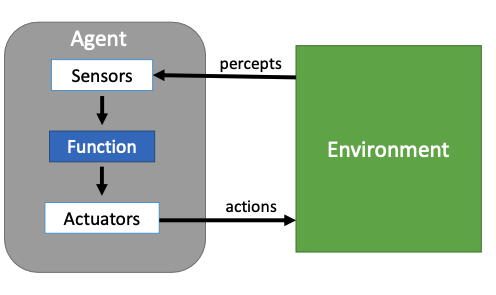
\includegraphics[width=0.7\linewidth]{1_PEAS.jpg}
    % \begin{itemize}
    %   \item \textbf{PEAS} 
    %   \begin{enumerate}
    %     \item \underline{Performance Measure:} Best for whom, what are we optimizing, what information is available, any unintended effects, what are the costs 
    %     \item \underline{Environment:} Refer to Environment section
    %     \item \underline{Actuators:} Allow intelligent agent to take actions or affect its environment
    %     \item \underline{Sensors:} Allow intelligent agent to perceive information about its environment 
    %   \end{enumerate}
    %   \item \textbf{Agent Function:} Maps from percept histories to actions, refer to Agent Function section
    % \end{itemize}
    
    % \subsection{Task Environment}
    % \begin{enumerate}
    %   \item \textbf{Fully Observable VS Partially Observable}
    %   \begin{itemize}
    %     \item \underline{Fully Observable:} Agent has complete \& accurate info about env state at all times (Eg. Chess)
    %     \item \underline{Partially Observable:} Agent has access to incomplete, uncertain or noisy info about env state (Eg. Self-driving cars)
    %   \end{itemize}
    %   \item \textbf{Deterministic VS Stochastic VS Strategic}
    %   \begin{itemize}
    %     \item \underline{Deterministic:} Next env state is completely determined by current state \& agent action $\vert$ Outcome is fully predictable (Eg. Sudoku)
    %     \item \underline{Stochastic:} Next env state is not completely determined by current state \& agent action $\vert$ Outcome is uncertain (Eg. Self-driving car)
    %     \item \underline{Strategic:} Env is deterministic, but outcomes depend on other agents' actions, requiring agent to consider strategies \& behaviors of others (Eg. Chess)
    %   \end{itemize}
    %   \item \textbf{Episodic VS Sequential}
    %   \begin{itemize}
    %     \item \underline{Episodic:} Agent actions are divided into discrete periods, each episode is independent of one another, agent makes decisions based on current episode (Eg. Classification task)
    %     \item \underline{Sequential:} Agent actions are inter-dependent, each action affects future states \& decisions, agent considers sequence of actions over time (Eg. Chess)
    %   \end{itemize}
    %   \item \textbf{Static VS Dynamic}
    %   \begin{itemize}
    %     \item \underline{Static:} Env state does not change while agent is deliberating
    %     \item \underline{Dynamic:} Env state changes over time even when agent is deliberating
    %     \item \underline{Semi-dynamic:} Env state does not change, but agent's performance score does
    %   \end{itemize}
    %   \item \textbf{Discrete VS Continuous}
    %   \begin{itemize}
    %     \item \underline{Discrete:} Finite \# of distinct, clearly defined percepts \& actions
    %     \item \underline{Continuous:} Infinite \# of percepts \& actions
    %   \end{itemize}
    %   \item \textbf{Single Agent VS Multi Agent}
    %   \begin{itemize}
    %     \item \underline{Single Agent:} Agent operating by itself in an env
    %     \item \underline{Multi Agent:} Multiple agents in an env
    %   \end{itemize}
    % \end{enumerate}

    % \subsection{Agent Structures}
    % \textit{Note: Agent is completely specified by Agent Function mapping percept sequences to actions}
    % \begin{enumerate}
    %   \item \textbf{Simple Reflex Agent:} Operates based on a set of predefined rules or conditions $\rightarrow$ Reacts to current state of env with a corresponding action $\rightarrow$ Does not have memory of past states or actions \& does not consider future consequences
    %   \item \textbf{Model-based Reflex Agent:} Extends simple reflex agent by maintaining internal model of world $\rightarrow$ Allows agent to keep track of current env state \& handle situations where env state is partially observable or changes over time
    %   \item \textbf{Goal-based Agent:} Operates with specific goals in mind $\rightarrow$ Selects actions based on ability to achieve these goals $\rightarrow$ Considers future \& plans its actions to achieve desired end state $\vert$ Uses goal representation \& perform search and planning
    %   \item \textbf{Utility-based Agent:} Extends goal based agent by considering not just whether goals are achieved, but how well they are achieved $\rightarrow$ Assigns utility value to different states \& chooses actions that maximize overall utility
    %   \item \textbf{Learning Agent:} Improves performance over time by learning from its experiences $\vert$ Can be reflex, model, goal \& utility based
    % \end{enumerate}
    % \begin{itemize}
    %   \item \textbf{Exploitation:} Maximize expected utility according to current knowledge about world
    %   \item \textbf{Exploration:} Trying to learn more about the world
    % \end{itemize}

    \section{Solving Problems by Searching}
    \subsection{Designing an Agent}
    \begin{itemize}
      \item \textbf{Assumptions:} Goal-based agent $\vert$ Env is fully observable, deterministic, static, discrete
      \item \textbf{Problem-solving Agent:} Agent that plans ahead (considers a seq. of actions that form a path to a goal state), undertakes SEARCH process
      \item \textbf{Steps:}
      \begin{enumerate}
        \item \underline{Goal Formulation:} \textit{(What do we want?)}
        \item \underline{Problem Formulation:} \textit{(How the world works?)} $\rightarrow$ States (state space), Initial State(initial state of agent), Goal State/Test (goal state of agent), Actions (things that agent can do in a given state), Transition Model (specifies outcome of an action to a given state \& how it leads to new states), Action Cost Function (cost of performing an action)
        \item \underline{Search:} \textit{(How to achieve it?)} $\rightarrow$ Path (seq. of actions), Solution (path to a goal)
        \item \underline{Execute}
      \end{enumerate}
      \item \textbf{Representation Invariant:} A condition that must be true over all valid concrete representations of a class
    \end{itemize}

    \subsection{Search Algorithms (Introduction)}
    \begin{itemize}
      \item \textbf{Search Algorithm:} Takes in search problem (input), returns solution/failure (output) $\vert$ Defined by Order of Expansion (FRONTIER)
      \item \textbf{Evaluation Criteria:}
      \begin{enumerate}
        \item \underline{Time Complexity:} \# of nodes generated/expanded
        \item \underline{Space Complexity:} Max \# of nodes in memory
        \item \underline{Completeness:} Does it return solution if it exists?
        \item \underline{Optimality:} Does it always find least cost solution?
      \end{enumerate}
      \begin{multicols}{2}
        \textbf{Tree Search:} 
        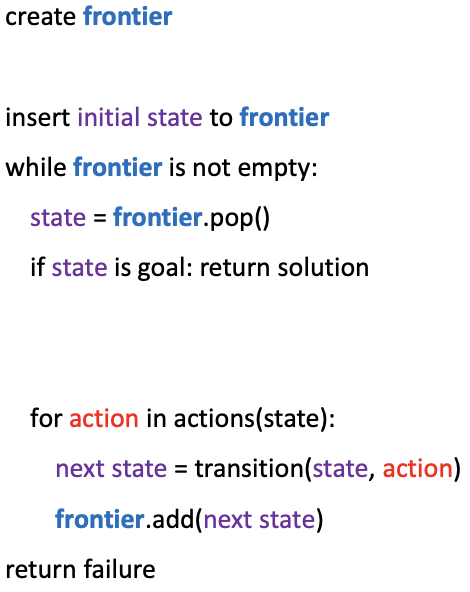
\includegraphics[width=0.75\linewidth]{2_tree_search.png}
        \\
        \columnbreak
        \textbf{Graph Search:}
        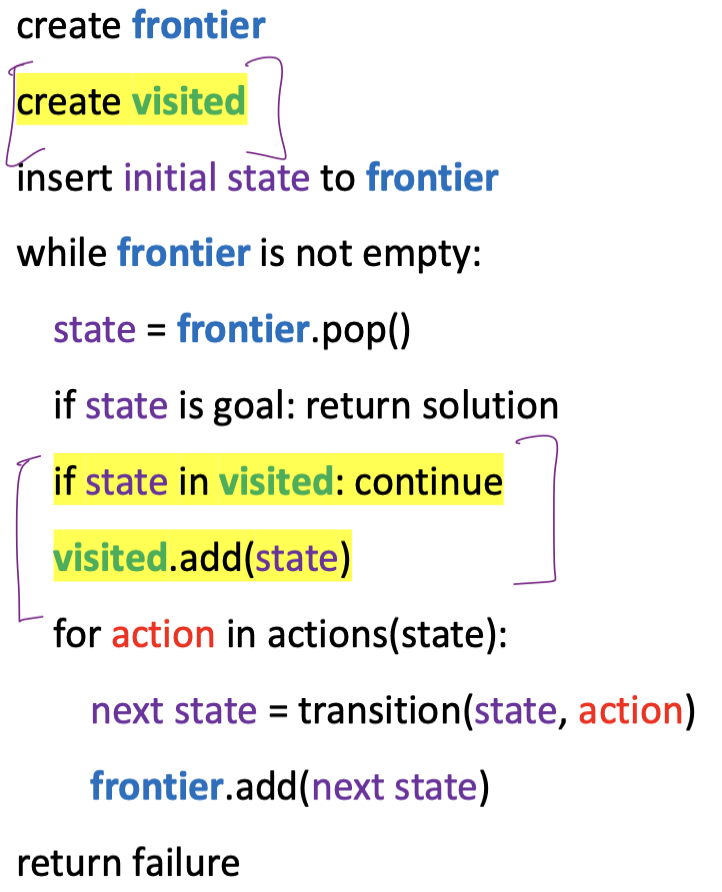
\includegraphics[width=0.75\linewidth]{3_graph_search.png}
      \end{multicols}
      \item \textbf{Checking of Goal State:}
      \begin{itemize}
        \item New state is checked for goal state before new states are PUSHED to frontier $\rightarrow$ Expand less states, may skip states with less cost
        \item State is checked for goal state after state is POPPED from frontier $\rightarrow$ Expand more states, will not skip states with less cost
      \end{itemize}
    \end{itemize}

    \subsection{Search Algorithms (Uninformed Search)}
    \begin{itemize}
      \item \textbf{Key Idea:} Search Algo is given no clue about how close a state is to the goal $\vert$ Can be Tree or Graph Search
      \item \textbf{BFS:} Queue Frontier $\vert$ Time Complexity: $O(b^d) = 1 + b + b^2 +$ $... + b^d$, where $b$ is branching factor, $d$ is depth of optimal solution $\vert$ Space Complexity: $O(b^d)$ when expanded until last child in worst case $\vert$ Completeness: Complete if $b$ is finite $\vert$ Optimality: Optimal if step cost is same everywhere
      \item \textbf{UCS:} Priority Queue (path cost) Frontier, where path cost == cost from root to a state $\vert$ Time Complexity: $O(b^{C^*/\epsilon})$, where $C^*$ is cost of optimal solution, $\epsilon$ is minimum edge cost $\rightarrow$ $C^*/\epsilon$ is est. depth of optimal solution in worst case $\vert$ Completeness: Complete if $\epsilon > 0$ and $C^*$ is finite (if $\epsilon = 0$, zero cost cycle may occur) $\vert$ Optimality: Optimal if $\epsilon > 0$
      \textit{Note: BFS is special case of UCS where step cost == 1 for every edge}
      \item \textbf{DFS:} Stack Frontier $\vert$ Time Complexity: $O(b^m)$ where $b$ is branching factor, $m$ is max depth $\vert$ Space Complexity: $O(bm)$ as only 1 path is expanded at one time $\vert$ Completeness: Not complete (when depth is infinite or can go back or forth) $\vert$ Optimality: Not optimal (there can be paths with less cost not explored yet)
      \item \textbf{DLS (Depth Limited Search):} Limit the search depth to $l$ where $l<=m$, backtrack once depth limit is reached $\vert$ Time Complexity: $O(b^l)$ $\vert$ Space Complexity: $O(bl)$ $\vert$ Completeness: Not complete when soln lies deeper $l$ $\vert$ Optimality: Not optimal when soln lies deeper than $l$
      \textit{Note: We dk the depth of solution, which is a downside}
      \item \textbf{IDS (Iterative Deepening Search):} Do DLS with max depth of $0,..,\infty$ $\rightarrow$ return soln if found, otherwise increase depth $\vert$ Time Complexity: $O(b^d)$, $Overhead=(n_{IDS} - n_{DLS})/n_{DLS}$ $\vert$ Space Complexity: $O(bd)$ $\vert$ Completeness: Complete $\vert$ Optimality: Optimal if step cost is same everywhere \\
      \textit{Note: IDS is not always faster than DFS $\rightarrow$ Consider state space s.t. each state have only single successor \& goal node is at depth $n$ $\rightarrow$ IDS will run in $O(n^2)$, DFS will run in $O(n)$}
      \item \textbf{Backward Search:} Search from goal
      \item \textbf{Bidirectional Search:} Combine forward search \& backward search, stop when 2 searches meet $\vert$ Time Complexity: $2*O(b^{d/2}) < O(b^d)$
    \end{itemize}

    \subsection{Search Algorithms (Informed Search)}
    \begin{itemize}
      \item \textbf{Key Idea:} Search Algo has a clue on how close a state is to the goal
      \item \textbf{Best First Search:} Priority Queue ($f(n)$) Frontier, where $f(n)$ estimates the goodness of a state (Node with lowest $f(n)$ is selected first to be expanded) $\vert$ $f(n)$ can be purely heuristic (estimated cost from $n$ to goal) or a combi of path cost \& heuristic
      \item \textbf{Greedy Best First Search:} Priority Queue ($f(n) = h(n)$) Frontier, where $h(n)$ is heuristic function that est. cost from $n$ to goal (Expands node that seems closest to goal according to $h(n)$ without considering path cost so far) $\vert$ Time Complexity: $O(b^m)$ $\vert$  Space Complexity: $O(b^m)$ $\vert$ Completeness: Not complete since GBFS might keep expanding nodes based on $h(n)$ without ever finding goal $\vert$  Optimality: Not optimal since GBFS selects nodes based on $h(n)$ without considering path cost
      \item \textbf{$A^*$ Search:} Priority Queue ($f(n) = g(n) + h(n)$) where $g(n)$ is cost so far to reach $n$ $\vert$ Time Complexity: $O(b^m)$ $\vert$ Space Complexity: $O(b^m)$ $\vert$  Completeness: Complete $\vert$ Optimality: Optimal
      \begin{itemize}
        \item If $h(n)$ is admissible $\rightarrow$ $A^*$ using Tree search is optimal
        \item If $h(n)$ is consistent $\rightarrow$ $A^*$ using Graph search is optimal
        \item \textit{Note: UCS is special case of $A^*$ search where $h(n) = 0$}
      \end{itemize}

      \subsection{Heuristics}
      \begin{itemize}
        \item Estimate cost from node $n$ to goal
        \item \textbf{Admissible Heuristics:} For every node $n$, $h(n) \leq h^*(n)$, where $h^*(n)$ is true cost to reach goal state from $n$ (Never over-estimate)
        \item \textbf{Consistent Heuristics:} For every node $n$, every successor $n'$ generated by action $a$, $h(n) \leq c(n,a,n') + h(n')$ and $h(G) = 0$ (Proof $h(n) - h(n') \leq c(n,a,n')$) \\
        \textit{Note: If $h(n)$ is consistent, $f(n') \geq f(n)$ $\rightarrow$ $f(n)$ is non-decreasing along any path $\rightarrow$ Nodes are expanded in order of increasing $f$ cost}
        \item \textbf{Dominance:} If $h_2(n) \geq h_1(n)$ for all $n$ $\rightarrow$ $h_2$ dominates $h_1$ $\vert$ If $h_2$ is admissible $\rightarrow$ $h_2$ is better for search
        \item \textbf{Creating Admissible Heuristics:}
        \begin{itemize}
          \item Problem with fewer restrictions on actions is called a relaxed problem
          \item Cost of an optimal soln to a relaxed problem is an admissible $h$ for original problem
        \end{itemize}
      \end{itemize}
    \end{itemize}

    \section{Local Search \& Adversarial Search}
    \subsection{Local Search}
    \begin{itemize}
      \item \textbf{Assumptions:} Agent is a Goal/Utility-based agent, Env has a very large state space
      \item \textbf{Informed \& Uninformed Search VS Local Search}
      \begin{enumerate}
        \item \underline{IUS:} Low to moderate state space $\vert$ Optimal or no soln $\vert$ Search path is usually the soln
        \item \underline{LS:} Very large state space $\vert$ Good enuf soln is preferable rather than no soln $\vert$ State is the soln (don't care about search path)
      \end{enumerate}
      \item \textbf{Local Search Overview:}
      \begin{itemize}
        \item \underline{Basic Idea:} Start somewhere in state space, move towards a better spot
        \item \underline{Problem Formulation:} States(state space), Initial State(initial state of agent), Goal test (optional, coz we actually dk the goal state, rely on eval function instead), Successor Function (possible states from a state), Evaluation Function (Output value/goodness of a state)
      \end{itemize}
      \item \textbf{Hill Climbing Algorithm}
      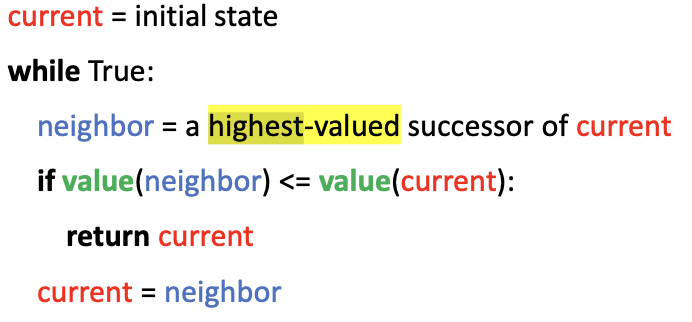
\includegraphics[width=0.75\linewidth]{4_hillclimbing.png}
      \begin{itemize}
        \item Known as Greedy Local Search (pick best amongst neighbors, repeat)
        \item \underline{Best Soln:} State space where eval. function has a max value (global max)
        \item \underline{Disadvantages:} Cannot reach global max if it enters local max, plateau $\vert$ Sensitive to choice of initial state, poor initial state may result in poor final state (Can overcome with random restarts, walks)
      \end{itemize}
      \item \textbf{Simulated Annealing}
      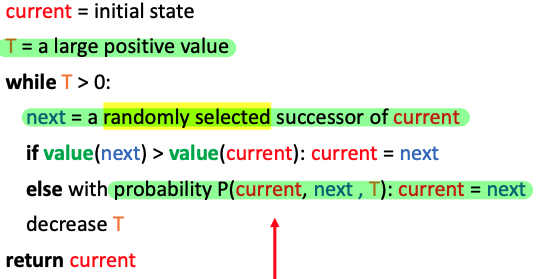
\includegraphics[width=0.75\linewidth]{5_simulated_annealing.png}
      \begin{itemize}
        \item P(current, next, T) = $e^{(value(next) - value(current))/T}$
        \item More exploration of bad states is allowed when $T$ is high, more exploitation is done when $T$ is low $\rightarrow$ basically choosing worse successor may lead to a better max
        \item \underline{Theorem:} If $T$ decreases slowly enough, SA will find global optimum with high probability
      \end{itemize}
    \end{itemize}

    \subsection{Adversarial Search}
    \begin{itemize}
      \item \textbf{Assumptions:} Agent is Utility-based $\vert$ Env is a game (game cannot be single player, partially observable, stochastic, but must be fully observable, deterministic, discrete, terminal states exist, 2 players, zero-sum, turn taking)
      \item \textbf{Minimax Algorithm:}
      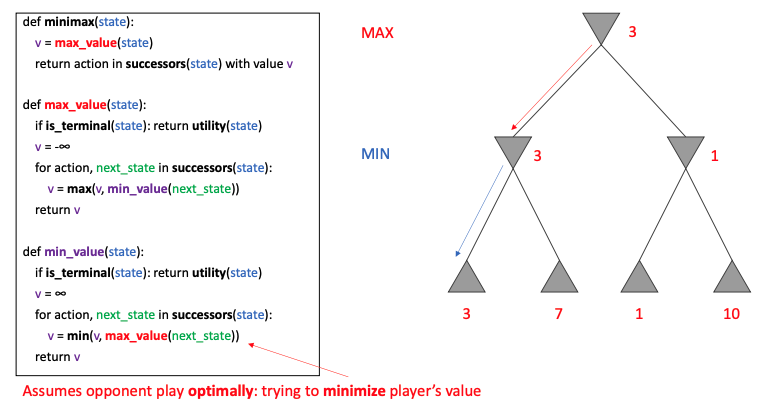
\includegraphics[width=0.9\linewidth]{6_minimax.png}
      \begin{itemize}
        \item \underline{Intuition:} MAX wins when utility is high, MIN wins when utility is low $\vert$ Assign utility values to all terminal states \& start tracing from terminal states $\rightarrow$ Eventually, all states will have utility values, starting player can choose a state that will max/min his utility
        \item \underline{Analysis:} Completeness: Complete if tree is finite $\vert$ Time Complexity: $O(b^m)$ $\vert$ Space Complexity: $O(bm)$ depth first exploration $\vert$ Optimality: Optimal against optimal opponent
      \end{itemize}
      \item \textbf{Alpha-beta Pruning}
      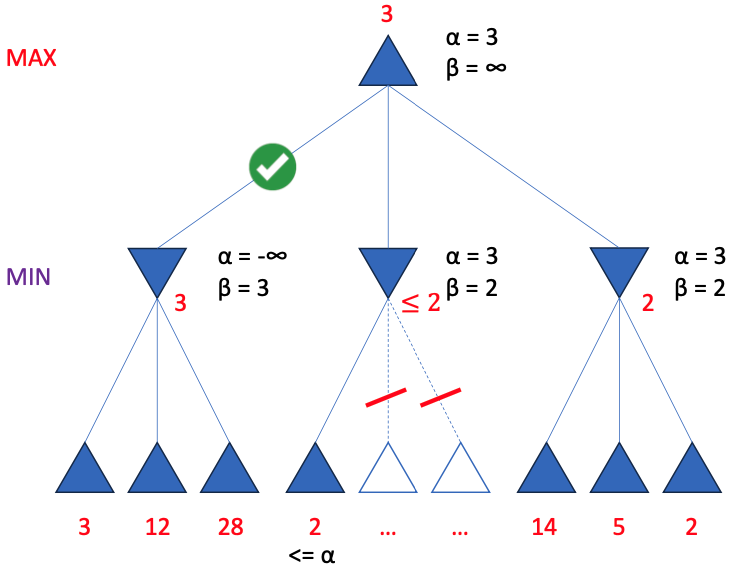
\includegraphics[width=0.75\linewidth]{7_alphabeta.png}
      \begin{itemize}
        \item \underline{Definitions:} $\alpha$ is best explored option to the root for MAX player (Highest value for MAX) $\vert$ $\beta$ is best explored option along path to the root for MIN player (Lowest value for MIN)
        \item \underline{Procedure:} 1. Assign $\alpha = -\infty, \beta = \infty$ for root 2. Propagate values down to the terminal node 3. Update $\alpha$ value at MAX node, $\beta$ value at MIN node 4. Propagate values up 5. Prune branches of nodes where $\alpha \geq \beta$
      \end{itemize}
      \item \textbf{Minimax with Cutoff}
      \begin{itemize}
        \item Instead of calling $is\_terminal$, call $is\_cutoff$ which returns TRUE if (1): State is terminal or (2): Cut-off is reached
        \item Instead of using $utility$, call $eval$ which is an eval. function that returns (1): Utility for terminal states or (2): Heuristic value for non-terminal states
      \end{itemize}
    \end{itemize}

    \section{Introduction to ML \& Decision Trees}
    \subsection{Introduction to ML}
    \begin{itemize}
      \item \textbf{Definitions:} Computer program is said to learn from experience $E$ w.r.t. some class of tasks $T$ \& performance measure $P$, if its performance at tasks in $T$, as measured by $P$, improves with experience $E$
      \item \textbf{Types of Feedback:}
      \begin{enumerate}
        \item \underline{Supervised Learning:} Involves training a model on a labeled dataset, where input data is paired with correct output $\rightarrow$ Model learns to map inputs to outputs based on this labeled data, allowing it to make predictions on new data
        \begin{itemize}
          \item \underline{Regression:} Predict continuous input
          \item \underline{Classification:} Predict discrete input
        \end{itemize} 
        \item \underline{Unsupervised Learning:} Deals with dataset that do not have labeled outputs $\rightarrow$ Goal is to identify patterns \& structures within data
        \item \underline{Reinforcement Learning:} Agent learns to make decisions by interacting with an environment $\rightarrow$ Agent receives feedback in the form of rewards or penalties based on its actions $\rightarrow$ Learns optimal behaviors over time
      \end{enumerate}
      \item \textbf{Formal Definitions:}
      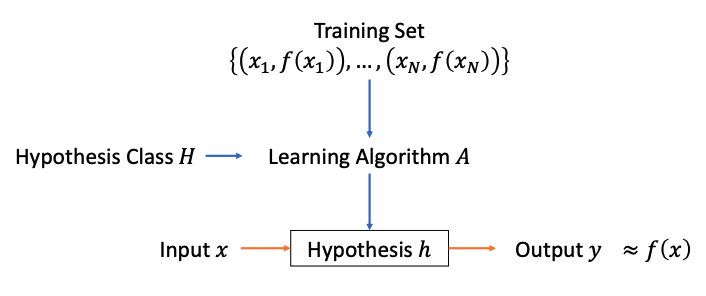
\includegraphics[width=0.75\linewidth]{8_ml_formal.png}
    \end{itemize}

    \subsection{Performance Measure}
    % \begin{itemize}
      % \item \textbf{Regression:} \\
      % 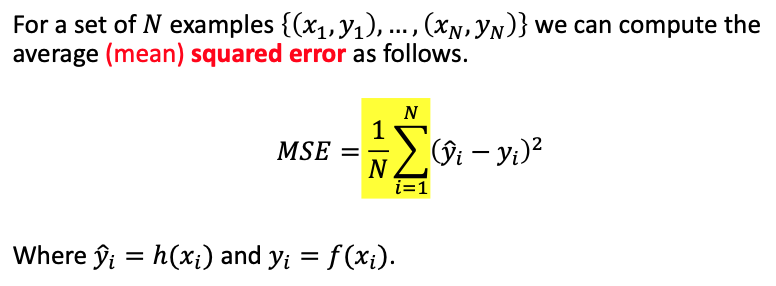
\includegraphics[width=0.75\linewidth]{9_mse.png}
      % 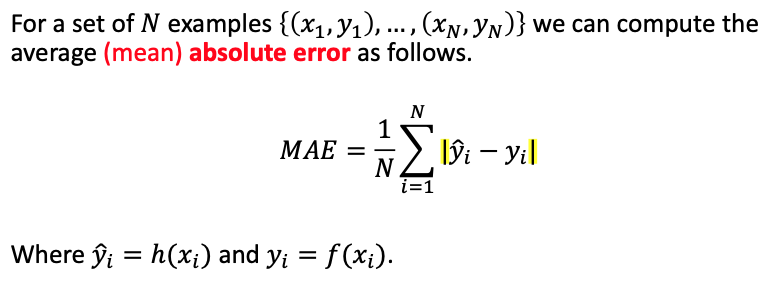
\includegraphics[width=0.75\linewidth]{10_mae.png}
      % \item \textbf{Classification:} \\
      % 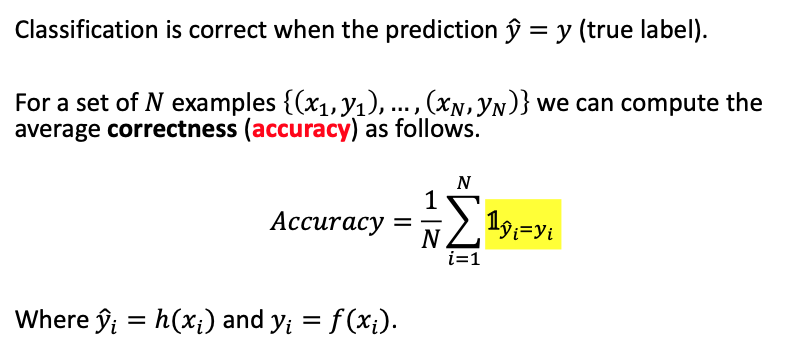
\includegraphics[width=0.75\linewidth]{11_accuracy.png}
      \begin{multicols}{2}
        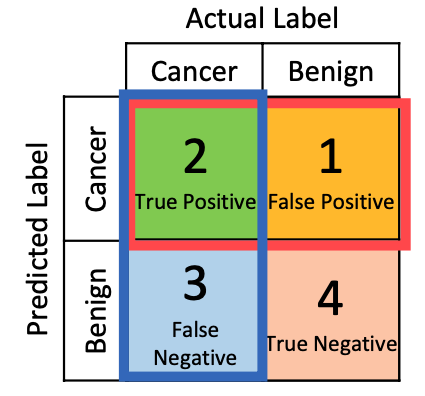
\includegraphics[width=0.8\linewidth]{12_confusion_matrix.png}
        \\
        \columnbreak
        \begin{itemize}
          \item \textbf{Accuracy:} $\frac{TP+TN}{TP+FN+FP+TN}$
          \item \textbf{Precision:} $\frac{TP}{TP+FP}$ (How many selected items are relevant, maximise if FP is costly)
          \item \textbf{Recall:} $\frac{TP}{TP+FN}$ (How many relevant items are selected, maximise if FN is dangerous)
          \item \textbf{F1 Score:} $\frac{2}{1/precision + 1/recall}$
        \end{itemize}
      \end{multicols}
    % \end{itemize}
    
    \subsection{Decision Trees}
    \begin{itemize}
      \item \textbf{Traits of Decision Trees:}
      \begin{itemize}
        \item Decision Trees can express any function of input attributes
        \item Consistent Decision Tree for any training set, but probably will not generalize to new examples
        \item \underline{\# of distinct decision trees with $n$ boolean attributes} = $2^{2^n}$
      \end{itemize}
      \item \textbf{Decision Tree Learning Algorithm}
      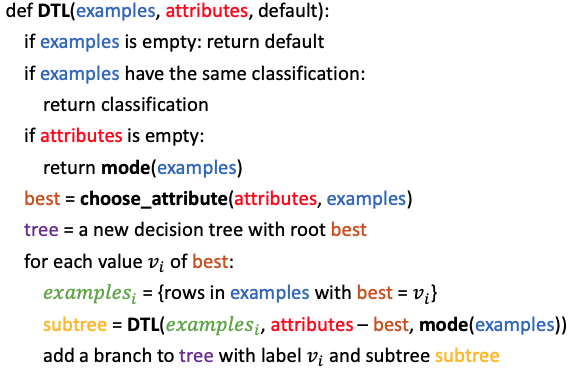
\includegraphics[width=0.8\linewidth]{13_decision_tree.png}
      \begin{itemize}
        \item \underline{mode:} Category with the highest number
        \item \underline{choose attribute:} Chooses attribute with the highest information gain
      \end{itemize}
      \item \textbf{Choosing an attribute:}
      \begin{itemize}
        \item Ideally select an attribute that splits examples into "all positive" or "all negative"
        \item \underline{Entropy} (Measure of randomness): $I(P(v_1),...,P(v_n)) = - \sum_{i=1}^{n}P(v_i)log_2P(v_i)$, where for data set containing $p$ positive \& $n$ negative examples, $I(\frac{p}{p+n}, \frac{n}{p+n}) = -\frac{p}{p+n}log_2\frac{p}{p+n}-\frac{n}{p+n}log_2\frac{n}{p+n}$ \\
        \textit{Note: I(1,0) = I(0,1) = 0, I(0.5, 0,5) = 1}
        \item \underline{Information Gain} (Entropy of curr. node - Total Entropy of children nodes): $IG(A) = I(\frac{p}{p+n}, \frac{n}{p+n}) - remainder(A)$ \\
        remainder(A) = $\sum_{i=1}^{v} \frac{p_i+n_i}{p+n} I(\frac{p_i}{p_i+n_i}, \frac{n_i}{p_i+n_i})$, where examples are split into $v$ subsets by attribute $A$
      \end{itemize}
      \item \textbf{Dealing with continuous valued attributes:} Define a discrete valued input attribute to partition values into discrete set of intervals
      \item \textbf{Dealing with missing values:} Assign most common value of attribute, assign probability to each value and sample, drop attribute, drop rows
      \item \textbf{Overfitting:} Decision Tree is perfect on training data, but worse on test data
      \item \textbf{Occam Razor:} Prefer short/simple hypothesis (long/complex hypothesis that fits data may be coincidence)
      \item \textbf{Pruning:} Prevents nodes from being split even when it fails to cleanly separate examples (Min samples leaf: Merge until leaf node is above min. samples number $\vert$ Max depth: Merge until leaf nodes are at depth less than max depth)
    \end{itemize}

    % \section{Tutorials Pointers}
    % \begin{itemize}
    %   \item \textbf{DFS:} DFS utilizes $O(bm)$ memory as DFS must store all nodes along the current path from root to the deepest node explored, along with branching factor $b$ at each level
    %   \item \textbf{UCS vs Dijkstra:} 2 algos are the same (both traverse search space in the manner, using a PQ to keep track of which nodes/states to visit next), but can argue that Dijkstra finds the shortest path to every node from a single source, while UCS only finds the shortest path to goal states
    % \end{itemize}

    % \section{Midterms PYP Pointers}
    % \begin{itemize}
    %   \item \textbf{Tree Search VS Graph Search:} Assuming the problem consists of discrete states (eg. pitcher problem), search space using tree search may be infinite (Eg. we keep filling up and emptying pitcher) $\rightarrow$ but using graph search will make search space finite (graph search will not revisit visited states)
    %   \item \textbf{Tree Search:}
    %   \begin{itemize}
    %     \item If optimal solution is needed: use BFS (for problems where each action has same cost), use UCS (for problems where each action has different cost), use IDS (if space is more important concern than time, since BFS is space inefficient)
    %     \item If optimal solution is not needed, but we need to preserve space: use DLS
    %     \item \underline{Termination \& Completeness on Tree Search Algorithms:}
    %     \begin{itemize}
    %       \item BFS is complete, but may not terminate
    %       \item DFS is incomplete and may not terminate
    %       \item UCS is complete, but may not terminate
    %       \item IDS is complete, but may not terminate (unless depth limiting condition is applied)
    %       \item DLS is complete and terminates regardless of whether a solution exists due to its depth limiting property
    %     \end{itemize}
    %   \end{itemize}
    %   \item \textbf{Heuristics:} 
    %   \begin{itemize}
    %     \item Max of 2 admissible heuristics ($max(h_0, h_1)$) for a problem is also an admissible heuristic $\rightarrow$ $max(h_0, h_1)$ is also dominant over $h_0$ \& $h_1$ since it takes max of both heuristics
    %     \item Given $h_0$ is admissible for problem $p_0$ \& $h_1$ is admissible for problem $p_1$ $\rightarrow$ $h_0$ \& $h_1$ are admissible for the combined problem $p_0 + p_1$ $\rightarrow$ $max(h_0, h_1)$ is also admissible and dominant for $p_0 + p_1$
    %     \item If heuristic is \textbf{consistent}, it must be \textbf{admissible} too!
    %     \item If heuristic is \textbf{non-admissible}, it must be \textbf{non-consistent} too!
    %     \item \underline{Common Proving Techniques:}
    %     \begin{itemize} 
    %       \item \textit{Consistency:} Decrease in heuristic value must not exceed action cost ($h(n) - h(n') \leq c(n,a,n')$) $\rightarrow$ Focus on maximum decrease in heuristic value and showing it is less than actual action cost
    %       \item \textit{Relaxed Problem:} True cost/admissible heuristic of a relaxed problem is an admissible heuristic to original problem, True cost of relaxed problem is consistent heuristic to original problem
    %     \end{itemize}
    %     \item \textbf{Dominance:} Not useful to describe dominance between non-admissible heuristics since non-admissible heuristics lead to sub-optimal search $\rightarrow$ for consistency sake, just treat it such that dominance concept can apply to both admissible \& non-admissible heuristics
    %   \end{itemize}
    % \end{itemize}

    % \subsection{Log Values (Base 2)}
    % \begin{enumerate}
    %   \item $log_21 = 0$
    %   \item $log_22 = 1$
    %   \item $log_23 = 1.58496$
    %   \item $log_24 = 2$
    %   \item $log_25 = 2.32192$
    %   \item $log_26 = 2.58496$
    %   \item $log_27 = 2.80735$
    %   \item $log_28 = 3$
    %   \item $log_29 = 3.16993$
    %   \item $log_210 = 3.32193$
    % \end{enumerate}

    \section{Linear Regression}
      \subsection{Linear Regression Basics}
        \begin{itemize}
          \item \textbf{Purpose:} Given $h_w(x) = w_0 + w_1x + ...$, find a $w$ that fits the data well
          \item \textbf{Mean Squared Error (Loss Function):} $J_{MSE}(w) = \frac{1}{2m}\sum^m_{ i=1}(h_w(x^{(i)})-y^{(i)})^2$
          \begin{enumerate}
            \item $m$ is the number of training examples
            \item $h_w(x^{(i)}) == \hat{y}^{(i)}$
            \item $y^{(i)}$ is actual $y$ value for the ith training example
          \end{enumerate}
          \item \textbf{Partial Derivative:} $\frac{\partial J_{MSE}(w)}{\partial w_1} = \frac{1}{m}\sum^m_{i=1}(w_1x^{(i)}-y^{(i)})x^{(i)}$ (when we differentiate $J_{MSE}(w)$ wrt. particiular weight, i.e. $w_1$)
        \end{itemize}
      
        \subsection{Gradient Descent}
        \begin{itemize}
          \item \textbf{Gradient Definition:} $\begin{bmatrix} \frac{\partial J(w)}{\partial w_0} \\ \frac{\partial J(w)}{\partial w_1} \\ ... \end{bmatrix}$, where each expression is a partial derivative wrt. different weights
          \item \textbf{Gradient Descent Algorithm:}
          \begin{enumerate}
            \item Start at some $w$
            \item Pick a nearby $w$ that reduces $J(w):$ $w_j \leftarrow w_j - \gamma \frac{\partial J(w_0, w_1, ...)}{\partial w_j}$
            \item Repeat until minimum is reached
          \end{enumerate}
          \item \textbf{Gradient Descent with 2 parameters:} Always store gradient in intermediate variable, then conduct gradient descent on each weight separately $\rightarrow$ Do not conduct gradient descent on all weights concurrently (or else a new weight will be updating another weight unknowingly)
          \item \textbf{Theorem:} $J_{MSE}(w)$ is convex for linear regression $\rightarrow$ 1 minimum, global minimum only
        \end{itemize}

        \subsection{Gradient Descent Variants}
        \begin{enumerate}
          \item \textbf{Batch Gradient Descent:} All training examples involved
          \item \textbf{Mini-batch Gradient Descent:} Subset of training examples at a time; Cheaper (faster); Random, may escape local minima for non-convex function
          \item \textbf{Stochastic Gradient Descent:} 1 random data point at a time (Order which we use the samples should be randomly decided); Cheapest (fastest); More random, may escape local minima for non-convex function
        \end{enumerate}

        \subsection{Extension of Linear Regression}
        \begin{itemize}
          \item \textbf{Features of different scales:} A feature with smaller magnitude will take much smaller steps each update than another feature with larger magnitude → Converging becomes slower
          \begin{enumerate}
            \item \underline{Solution 1:} Have different learning rates for each weight
            \item \underline{Solution 2:} Conduct mean normalization $x_j \leftarrow \frac{x_j-\mu_j}{\sigma_j}$, where $\sigma_j$ is the standard deviation of the feature across all training examples \& $\mu_j$ is the mean of the feature across all training examples
          \end{enumerate}
          \item \textbf{Non-linear relationship:} Use polynomial regression for non-linear relationship (transform features) $|$ Terms that are raised to a power more than 1 might need to be scaled as they can become too big $|$ Max degree of polynomial needed to fit any set of $n$ points is $n-1$ (otherwise will overfit)
        \end{itemize}

        \subsection{Normal Equation}
        \begin{itemize}
          \item \textbf{Normal Equation Procedure:}
          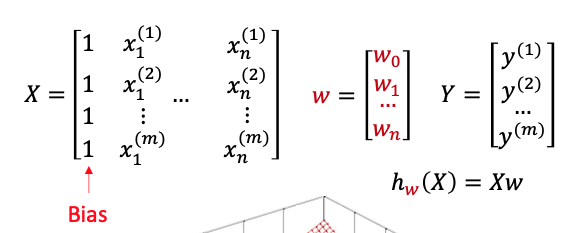
\includegraphics[width=0.6\linewidth]{16_matrices.png}
          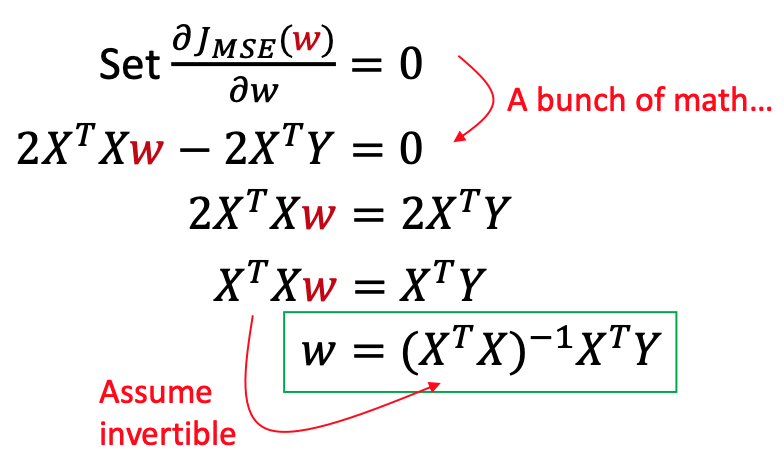
\includegraphics[width=0.45\linewidth]{17_normal_equation.png} \\
          $X^TX$becomes non-invertible when it is singular, which occurs when its rows (repeated or identical data points) or columns (redundant or highly correlated features) are linearly dependent
          \item \textbf{Gradient Descent VS Normal Equation:}
          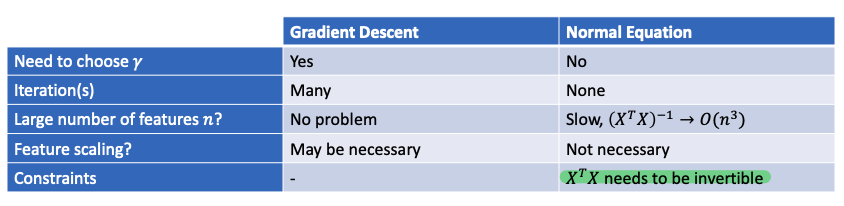
\includegraphics[width=0.8\linewidth]{18_comparision.png}
        \end{itemize}

        \section{Logistic Regression}
        \subsection{Logistic Regression Basics}
        \begin{itemize}
          \item Used for classification problems 
          \item \textbf{Logistic Regression (1D)}
          \begin{itemize}
            \item \underline{Logistic Function:} $\sigma(z) = \frac{1}{1 + e^{-z}}$, where $z = wx$
            \item Output of $\sigma(z)$ aka. $h_w(x)$ is in [0,1] and treated as a probability $\rightarrow$ If $\sigma(z)>\alpha$, then label as 1
          \end{itemize}
          \item \textbf{Logistic Regression (2D):} Decision boundary is a line of intersection between prediction boundary plane and plane containing all the prediction points $\rightarrow$ Decision boundary is perpendicular to $w$
        \end{itemize}

        \subsection{Measuring Fit}
        \begin{itemize}
          \item \textbf{Why MSE is bad for Logistic Regression:} $J_{MSE}$ for logistic regression would not work well as it is non-linear $\rightarrow$ non-convex $\rightarrow$ multiple local minima
          \item \textbf{Cross Entropy for $C$ classes:} $CE(y, \hat{y}) = \sum_{i=1}^C -y_ilog(\hat{y}_i)$ (Measures the average number of bits required to identify an event from 1 probability distribution → measures the difference between discovered probability distribution of a classification model \& predicted values)
          \item \textbf{Binary Cross Entropy for 2 classes:} $BCE(y, \hat{y}) = -ylog(\hat{y}) -(1-y)log(1-\hat{y})$
          \begin{enumerate}
            \item Given $y=1$ \& value of $\hat{y}$ is high, model will be rewarded for making a correct prediction
            \item Given $y=1$ \& value of $\hat{y}$ is low, model will be penalized for making a wrong prediction
          \end{enumerate}
          \item \textbf{BCE Loss Function:} $J_{BCE}(w) = \frac{1}{m}\sum^m_{i=1}BCE(y^{(i)}, h_w(x^{(i)}))$, which is convex for logistic regression $\rightarrow$ Can find global minimum during gradient descent
        \end{itemize}

        \subsection{Gradient Descent}
        \begin{itemize}
          \item \textbf{Partial Derivative:} $\frac{\partial J_{BCE}(w)}{\partial w_0} = \frac{1}{m} \sum_{i=1}^{m} \left( h_w(x^{(i)}) - y^{(i)} \right)$ \\ $\frac{\partial J_{BCE}(w)}{\partial w_1} = \frac{1}{m} \sum_{i=1}^{m} \left( h_w(x^{(i)}) - y^{(i)} \right) x_1^{(i)}$
        \end{itemize}

        \subsection{Multi-Class Classification}
        \begin{itemize}
          \item Split the multi-class dataset into multiple binary classification problems $\rightarrow$ Binary classifier is then trained on each binary classification problem \& predictions are made using the model that is the most confident
          \item \textbf{One VS All}: Fit 1 classifier per class, fit against all other classes $\rightarrow$ Pick the highest probability (Eg. 3 classes of cat, dog, rabbit $\rightarrow$ Classifier of cat against all other classes gives the highest probability $\rightarrow$ Predict as cat)
          \item \textbf{One VS One}: Fit 1 classifier per class pair $\rightarrow$ Pick the most wins (Eg. Cat wins Dog, Rabbit wins Cat, Rabbit wins Dog $\rightarrow$ Predict as Rabbit)
        \end{itemize}

        \subsection{Performance Measure}
        \begin{itemize}
          \item \textbf{True Positive Rate \& False Positive Rate:} $TPR = \frac{TP}{TP+FN}, FPR = \frac{FP}{FP+TN}$
          \item \textbf{Receiver Operator Characteristics (ROC) Curve:}
          \begin{itemize}
            \item Graphical plot that illustrates performance of a binary classifier
            \item Different data plots are for different $\alpha$ threshold values
            \item If ROC curve is above diagonal random line $\rightarrow$ Model is more accurate than random chance
            \item \underline{Area under curve (AUC) of ROC:} AUC $>$ 0.5 means model is better than chance, AUC $\approx$ 1 means model is very accurate, AUC = 0 means model is predicting opposite class for each data
          \end{itemize}
          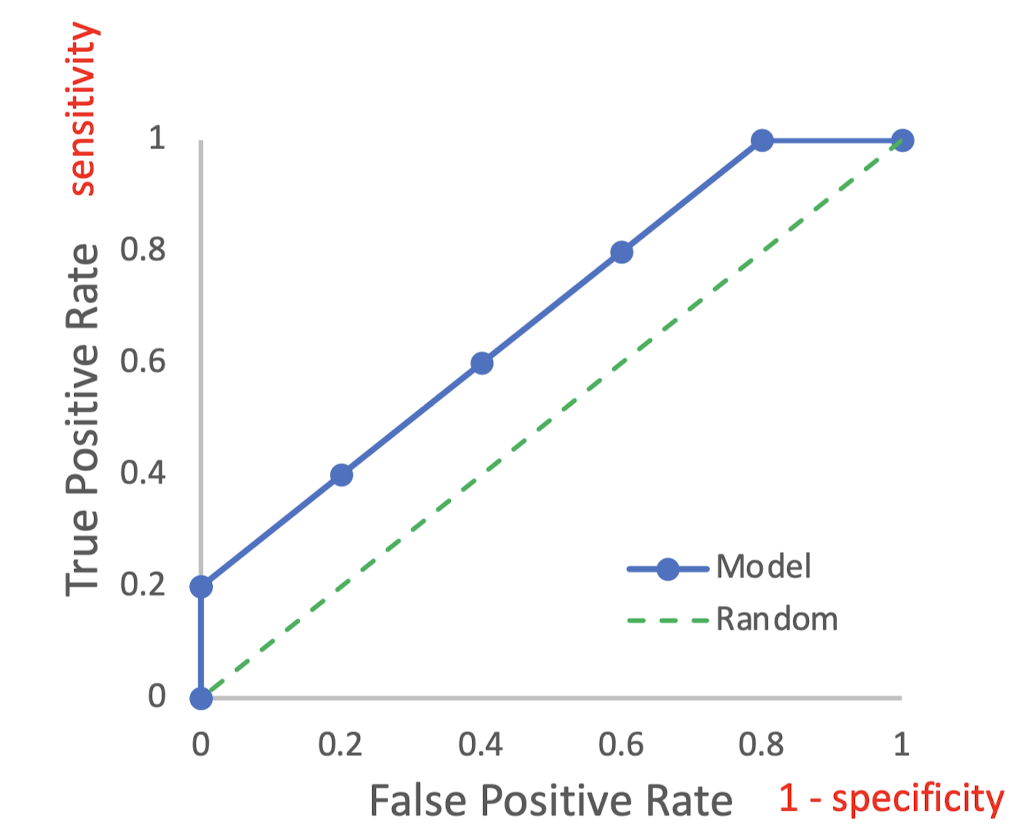
\includegraphics[width=0.6\linewidth]{19_ROC.png}
        \end{itemize}

        \subsection{Model Evaluation \& Selection, Hyper-parameter Tuning}
        \begin{itemize}
          \item \textbf{Model Selection (based on error function):}
          \begin{enumerate}
            \item Train each model $h_i$ on training set $D_{train}$
            \item Run the models on validation set $D_{val}$ $\rightarrow$ Choose model with MINIMUM $J_{D_{val}}$
            \item Test that model on a test set $D_{test}$ \& assess the model by computing $J_{D_{test}}$
          \end{enumerate}
          \item \textbf{Model Evaluation:} When comparing a logistic regression model's output with target label, use Accuracy or AUC-ROC, but not loss functions such as MSE, MAE, BCE
          \item \textbf{Bias:} Error introduced by approximating a real-world problem (which may be very complex) with a simplified model $\rightarrow$ High bias is associated with Under-fitting \& perform poorly on both training and test data
          \item \textbf{Variance:} Error introduced by the model's sensitivity to small fluctuations in the training data $\rightarrow$ High variance is associated with Over-fitting \& Perform well on the training data but poorly on test data
          \item \textbf{Hyperparameter Tuning:} To find the best model by looping through:
          \begin{enumerate}
            \item Pick hyperparameters (Eg. Learning rate of gradient descent, max depth of decision tree, min sample of decision tree, loss function of regression model)
            \item Train model with hyperparameters
            \item Evaluate model
          \end{enumerate}
        \end{itemize}

        \section{Support Vector Machine}
        \subsection{Regularisation}
        \begin{itemize}
          \item \textbf{Methods to address overfitting}
          \begin{enumerate}
            \item Reduce number of features from high degree to low degree polynomial
            \item \underline{Regularisation}: Keep all features but reduce magnitude of $w_j \rightarrow$ Done by adding the weights to cost function, but since we do not know which $w_j$ to penalise, we penalise all $w_j$ instead 
          \end{enumerate}
          \item \textbf{Linear Regression with Regularisation}
          \begin{itemize}
            \item \underline{Cost Function:} $J(w) = \frac{1}{2m} \sum_{i=1}^{m} \left( h_w(x^{(i)}) - y^{(i)} \right)^2 + \frac{\lambda}{2m} \sum_{j=1}^{n} w_j^2$
            \item \underline{Gradient Descent:} $w_j \leftarrow w_j - \gamma \frac{1}{m} \sum_{i=1}^{m} \left( h_w(x^{(i)}) - y^{(i)} \right) x_j^{(i)} - \gamma \frac{\lambda}{m} w_j$
            \item When $\gamma = 0$, there is no regularisation, overfitting occurs
            \item When $\gamma = $ high value, there is too much regularisation, under fitting occurs (line equation reduces to just $w_0$) 
          \end{itemize}
          \item \textbf{Linear Regression with Regularisation (Normal Equation)}
          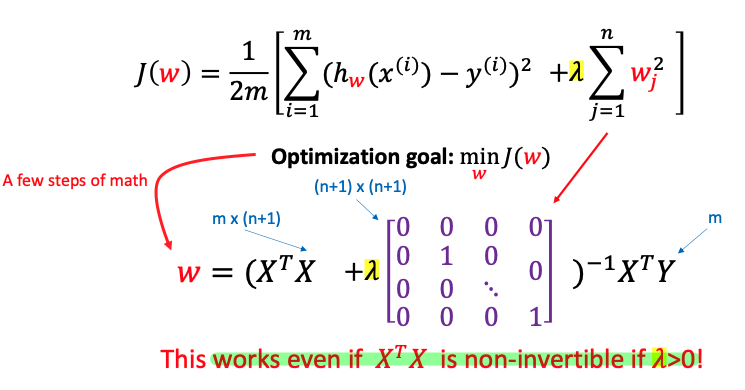
\includegraphics[width=0.7\linewidth]{20_regularisation_normal_equation.png}
          \begin{itemize}
            \item Modify the regularisation matrix such that the 1st element (corresponding to bias term) is 0 instead of 1 → 1st row and column correspond to bias term $w_0$ and are set to 0 to not penalise the bias term
          \end{itemize}
          \item \textbf{Logistic Regression with Regularisation}
          \begin{itemize}
            \item \underline{Cost Function:} $J(w) = -\frac{1}{m} \sum_{i=1}^{m} [ y^{(i)} \log h_w(x^{(i)}) +\left( 1 - y^{(i)} \right) \log \left( 1 - h_w(x^{(i)}) \right)] + \frac{\lambda}{2m} \sum_{j=1}^{n} w_j^2$
            \item \underline{Gradient Descent:} $w_j \leftarrow w_j - \gamma \frac{1}{m} \sum_{i=1}^{m} \left( h_w(x^{(i)}) - y^{(i)} \right) x_n^{(i)} - \gamma \frac{\lambda}{m} w_j$
          \end{itemize}
        \end{itemize}

        \subsection{Support Vector Machine}
        \begin{itemize}
          \item \textbf{Background:} We want to maximise the margin between all positive \& negative points
          \item \textbf{Procedure (Hard Margin SVM):}
          \begin{enumerate}
            \item Define decision rule (what is positive point, what is negative point): $\vec{w} \cdot \vec{x} + b \geq 0$ then positive
            \item Equation of margin: $margin = \frac{2}{||w||}$
            \item Constrained Optimization Problem: $\min \frac{1}{2} \|\mathbf{w}\|^2 \quad \text{s.t.} \quad y^{(i)} \left( \mathbf{w} \cdot \mathbf{x}^{(i)} + b \right) - 1 \geq 0$ \\ or \\ $\max_{\alpha \geq 0} \sum_{i} \alpha^{(i)} - \frac{1}{2} \sum_{i} \sum_{j} \alpha^{(i)} \alpha^{(j)} y^{(i)} y^{(j)}  \left( \mathbf{x}^{(i)} \cdot \mathbf{x}^{(j)} \right)$
            \item Parameterization of decision boundary: Form system of equations using constraints and equation for the weights ($\sum_{i=1}^n\alpha^{(i)}y^{(i)}=0$ and $w=\sum_{i=1}^n\alpha^{(i)}y^{(i)}x^{(i)}$) $\rightarrow$ Obtain values of $\alpha^{(i)}$ with GJE
            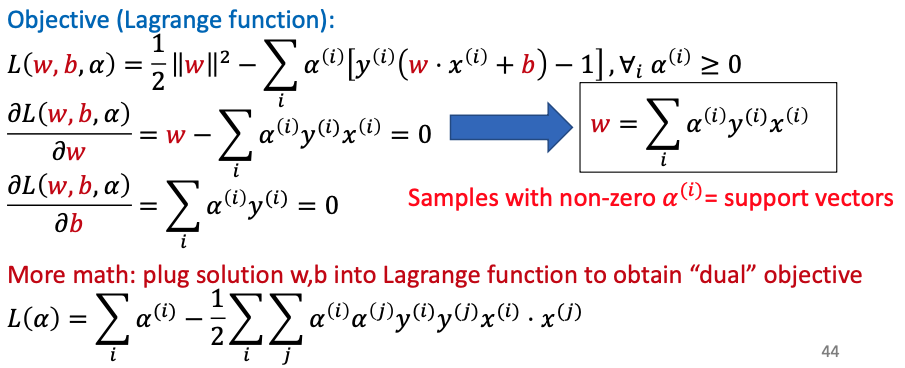
\includegraphics[width=0.85\linewidth]{25_lang_func.png}
          \end{enumerate}
          \item \textbf{Soft Margin SVM}
          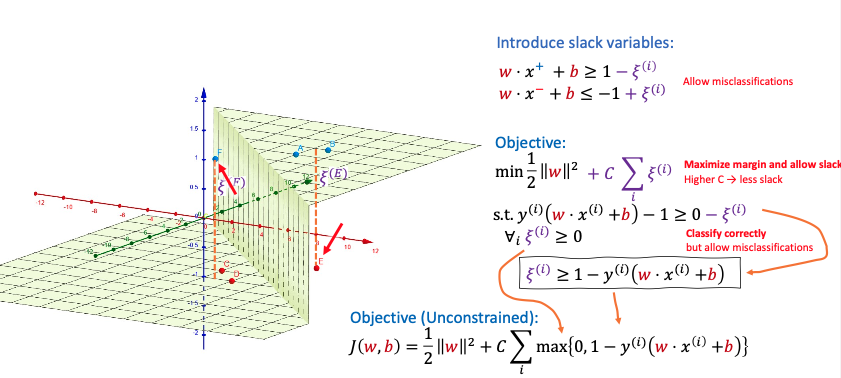
\includegraphics[width=0.95\linewidth]{21_softmargin.png}
          \begin{itemize}
            \item Soft margin SVM is used when data is not linearly separable (allows for some misclassification of training data)
            \item Slack variable is introduced to handle instances where data points are either on wrong side of margin or even misclassified
            \begin{enumerate}
              \item $\xi_i = 0$ means data point lies either on or outside margin \& is correctly classified
              \item $0 < \xi_i \leq 1$ means data point is within margin, but still correctly classified
              \item $\xi_i > 1$ means data point is on wrong side of decision boundary (misclassified)
            \end{enumerate}
            \item $C$ is regularisation parameter that controls the trade-off between maximising the margin and minimising classification errors → Larger $C$ gives more importance to minimising slack variables (fewer misclassifications are allowed), while smaller C allows for more margin violations
          \end{itemize}
          \item \textbf{Kernel Methods \& Kernel Tricks}
          \begin{itemize}
            \item Used when data is truly not linearly separable
            \item Use a kernel to transform data into higher dimensional space for non-linearly separable data
          \end{itemize}
        \end{itemize}

        \section{Introduction to Neural Networks}
        \subsection{Perceptron}
        \begin{itemize}
          \item \textbf{Formula:} $\hat{y} = h_w(x) = g(\sum_{i=0}^n w_ix_i)$, where $g$ is the activation function \& $g$ is normally the sign function ($g(z) = +1 if z \geq 0, else -1$) for perceptrons
          \item \textbf{Perceptron Learning Algorithm:}
          \begin{enumerate}
            \item Initialise $\forall_iw_i$ (set random initial weights)
            \item Loop (until convergence aka. no misclassification or max steps reached)
            \begin{itemize}
              \item For each instance $(x^{(i)}, y^{(i)})$, classify $\hat{y}^{(i)} = h_w(x^{(i)})$
              \item Select 1 misclassified instance $(x^{(j)}, y^{(j)})$
              \item Update weights: $w \leftarrow w + \gamma(y^{(j)} - \hat{y}^{(j)})x^{(j)}$ (remember to add bias term for $x$)
            \end{itemize}
          \end{enumerate}
        \end{itemize}

        \subsection{Neural Networks}
        \begin{itemize}
          \item \textbf{Single Layer Neural Network} 
          \begin{itemize}
            \item Same like perceptron, except $g$ is normally non-linear (Eg. $\sigma$, tanh, ReLU, Leaky ReLU)
            \item NOT, AND, OR, NOR functions can be modelled by single layer, but XOR, XNOR require multi-layer (data is not linearly seprable)
          \end{itemize}
          \item \textbf{Matrix multiplication in Neural Network:} $\hat{y} = g(W^Tx)$ in a single layer, where \# of rows in $W$ == \# of inputs per perceptron, \# of columns in $W$ == \# of perceptrons in layer
          \item \textbf{Forward Propagation across multi-layer:} Basically repeated matrix multiplication from right to left
          \item \textbf{Regression \& Classification}
          \begin{itemize}
            \item Activation function of perceptron(s) in final layer determines if we are doing regression (linear/no activation), binary classification (sigmoid) or multi-class classification (softmax)
            \item \underline{Softmax activation:} $g(z) = \frac{e^{z_i}}{\sum_{j=1}^Ce^{z_j}}$, where sum of outputs of all the final layer perceptrons is 1
          \end{itemize}
        \end{itemize}

        \subsection{Gradient Descent with Neural Network}
        \begin{itemize}
          \item \textbf{Derivative of Sigmoid function:} $\sigma(x) = \frac{1}{1 + e^{-x}}$, $\sigma'(x)=\sigma(x)(1-\sigma(x))$
          \item \textbf{Gradient Descent on Single layer Neural Network:} Given $a = \sum_{i=0}^nw_ix_i$, $\hat{y}=\sigma(a)$, $L = \frac{1}{2}(\hat{y} - y)^2$ (MSE), Weight update is $w_i \leftarrow w_i - \gamma\frac{dL}{dw_i}$ == $w_i \leftarrow w_i - \gamma(\hat{y}-y)\hat{y}(1-\hat{y})x_i$ (Derived with chain rule)
        \end{itemize}

        \subsection{Neural Network VS Other models}
        \begin{enumerate}
          \item \textbf{Logistic Regression:} Has Linear, Non-robust decision boundary (prone to misclassification since decision boundary can be too close to data points)
          \item \textbf{Logistic Regression with Feature Mapping:} Has Non-linear, Non-robust decision boundary (prone to misclassification since decision boundary can be too close to data points)
          \item \textbf{Support Vector Machine:} Has Non-linear, Robust decision boundary (decision boundary is guaranteed to be far from data points)
          \item \textbf{Neural Networks:} Has Non-linear, non-robust decision boundary (prone to misclassification since decision boundary can be too close to data points)
        \end{enumerate}

        \subsection{Back Propagation}
        \begin{itemize}
          \item \textbf{Chain Rule Background:}
          \begin{enumerate}
            \item \underline{1 intermediate variable:} Given $a=f(x), z=g(a)$, then $\frac{dz}{dx} = \frac{dz}{da}\frac{da}{dx}$
            \item \underline{2 intermediate variables:} Given $a=f(x), b=g(x), z=h(a,b)$, then $\frac{dz}{dx} = \frac{dz}{da}\frac{da}{dx} + \frac{dz}{db}\frac{db}{dx}$
          \end{enumerate}
          \item \textbf{Back Propagation with Linear Activation:}
          \begin{itemize}
            \item Given linear activation $g(x)=x$ and loss function $L=\frac{1}{2}(\hat{y} - y)^2$
            \item Do 1 round of forward propagation first, get the all the nodes' values $(v_i, u_i)$ first
            \item Do 1 round of back propagation next (RIGHT TO LEFT), calculating all the $\frac{dL}{da_i}$ then $\frac{dL}{dw_i}$ and then updating the weights via $w_i \leftarrow w_i - \gamma \frac{dL}{dw_i}$ \\
            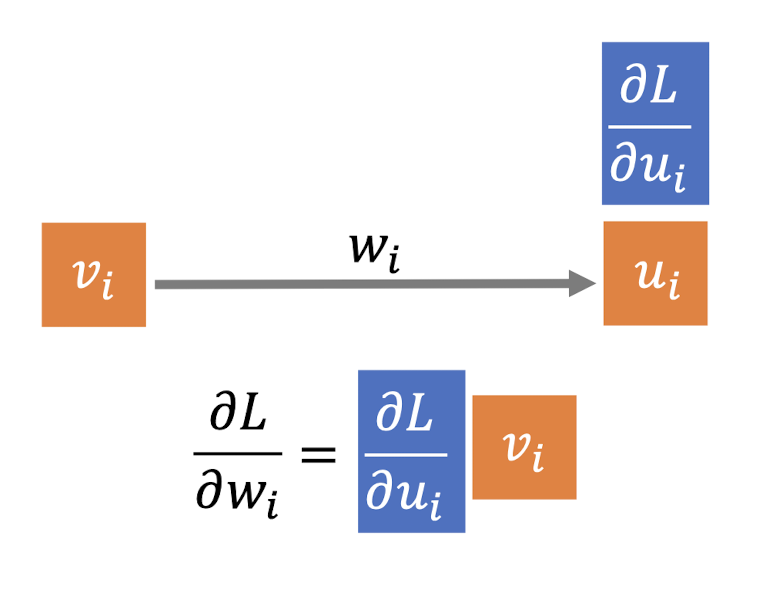
\includegraphics[width=0.5\linewidth]{22_backprop_single_unit.png}
            \item $\frac{dL}{dw_i}=\frac{dL}{du_i}\frac{du_i}{dw_i}=\frac{dL}{du_i}v_i$
            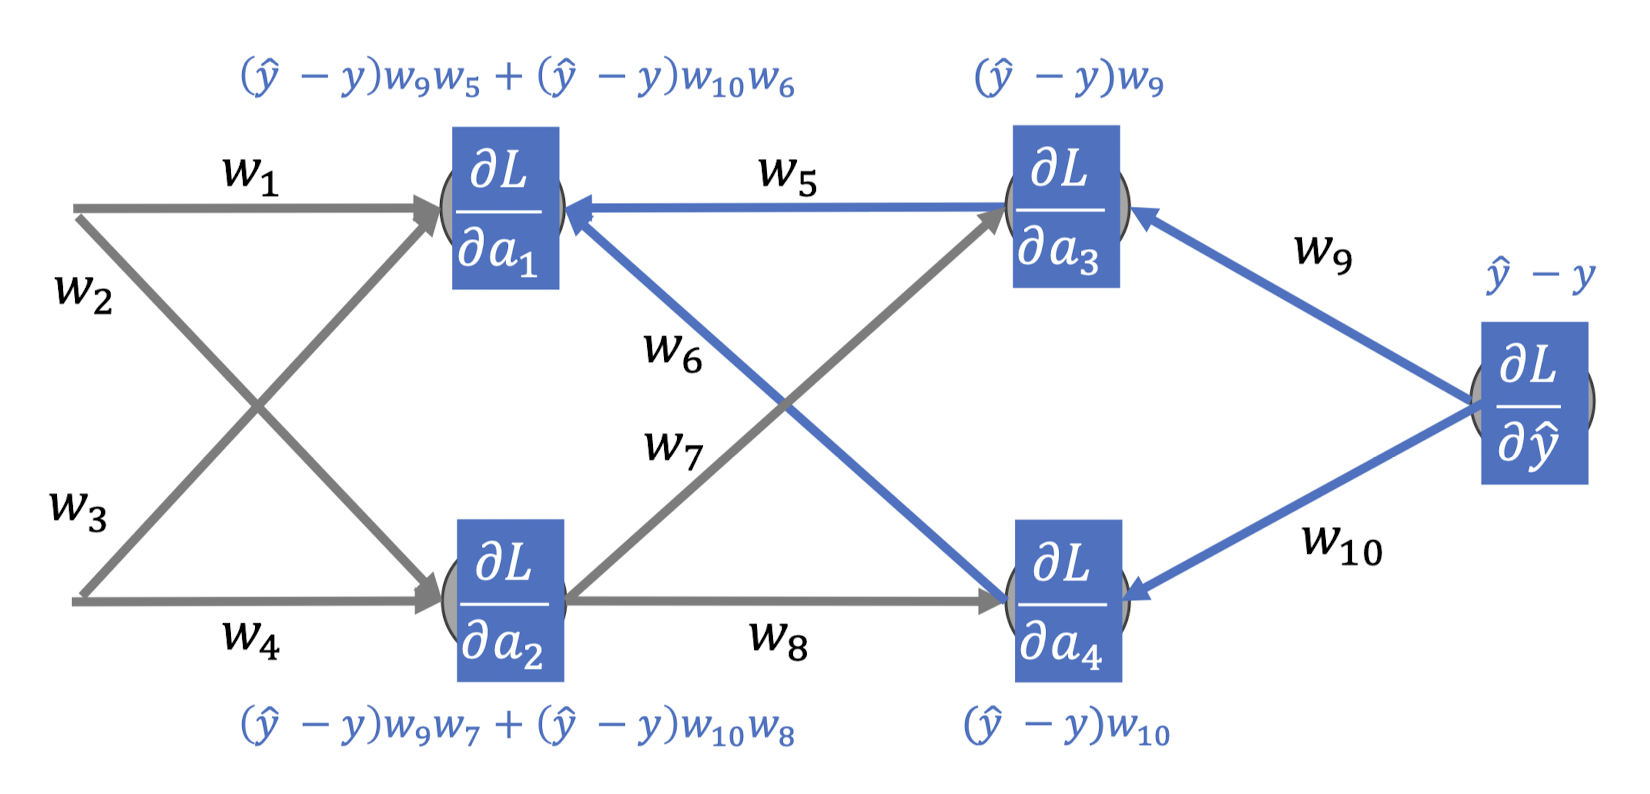
\includegraphics[width=0.7\linewidth]{23_backprog_linear.png}
          \end{itemize}
          \item \textbf{Back Propagation with Non-linear Activation:}
          \begin{itemize}
            \item Given non-linear activation $g(x)$ and loss function $L=\frac{1}{2}(\hat{y} - y)^2$
            \item Same as linear activation, except need to account for $g'(z_i)$
            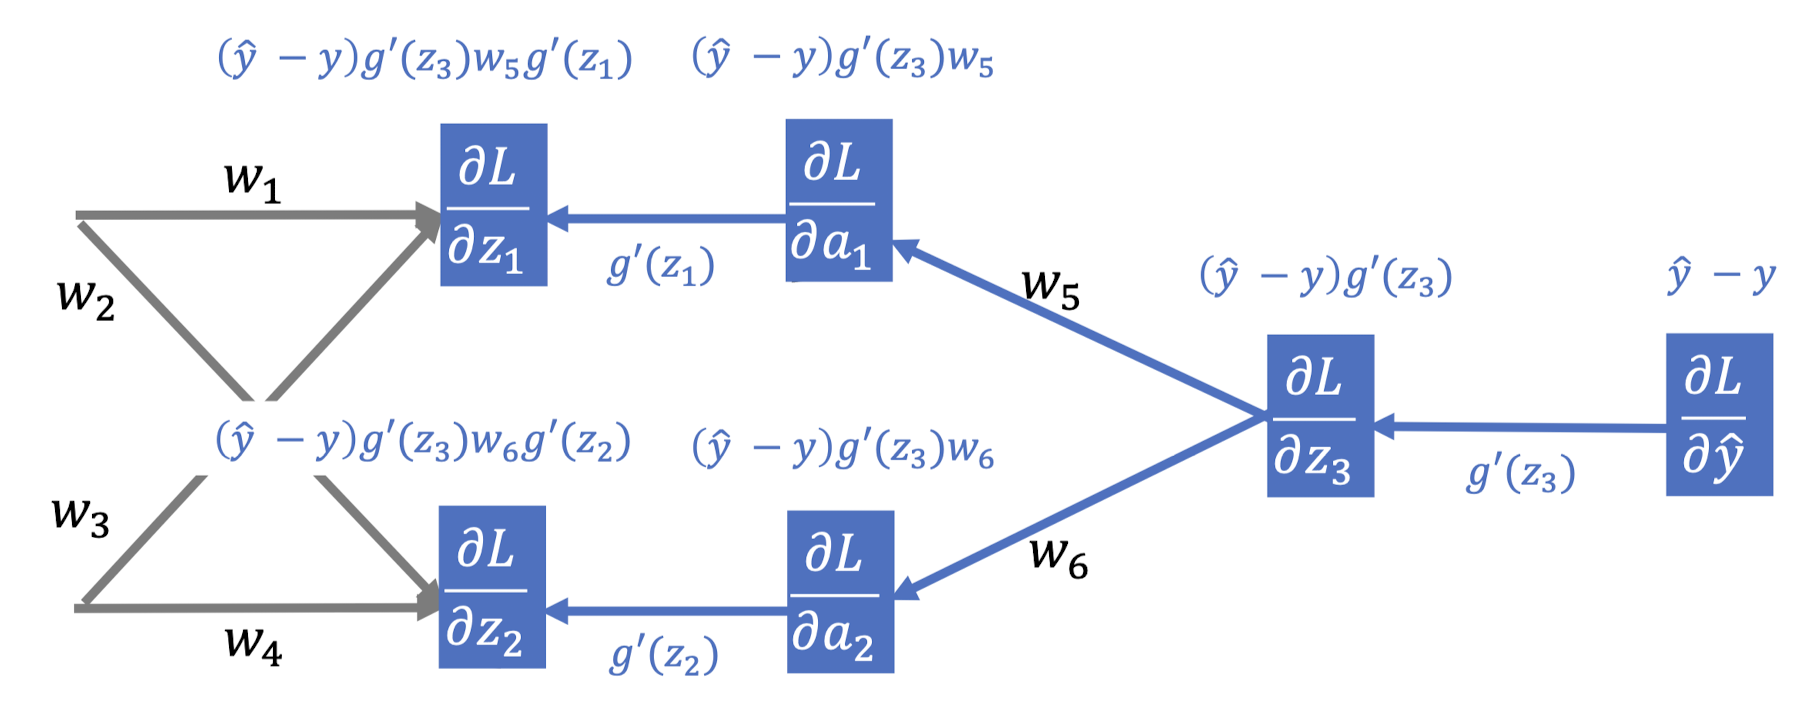
\includegraphics[width=0.75\linewidth]{24_backprog_non_linear.png}
          \end{itemize}
        \end{itemize}

        \section{Convolution Neural Network}
        \subsection{Purpose}
        \begin{itemize}
          \item Automatically \& efficiently learn features from data while maintaining spatial relationships between pixels
          \item Does not make sense to have $800\times800\times100$ = 64 million weights for a neural network with 100 neurons for a $800\times800$ input pixel image $\rightarrow$ Use CNN instead
        \end{itemize}
        
        \subsection{Convolution:2D}
        \begin{itemize}
          \item Given image input $X$ and kernel $W$ $\rightarrow$ Multiply sliding input window with kernel then sum $\rightarrow$ Output a feature map
          \item If we want to detect 1 more feature, we use another kernel and form another feature map
        \end{itemize}

        \subsection{Convolution Tricks}
        \begin{itemize}
          \item \textbf{Add Padding:} Add padding of 0s to image input $\rightarrow$ Resulting feature map can be same size as original image input $\rightarrow$ Without padding, size of feature maps would shrink with each layer, which could lead to loss of important information, especially near the edges of the image
          \item \textbf{Add Strides:} Increase stride length, so that we slide the input window multiple pixels over a single step $\rightarrow$ Reduces the size of feature maps (manage computational costs) $\rightarrow$ Larger stride focuses on more global patterns rather than small, localized details (reduces risk of overfitting)
          \item \textbf{Formula to get dimension of feature map:} Output Dimension = [(Input Dimension - Kernel Dimension + 2 * Padding) / Stride] + 1
          \item \textbf{Pooling layer:} Down-samples feature maps via Max pool, Average pool, Sum pool
          \item \textbf{Receptive Field:} Area of the input that contributes the output of a neuron in a convolutional layer (gives us an idea of where we are getting our results from as data flows through the layers of the network) $\rightarrow$ Larger receptive field enables network to capture more global features
          \begin{enumerate}
            \item Let $r_0=1, j_0=1$
            \item $r_i=r_{i-1} + (kernel_i - 1)\times j_{i-1}$
            \item $j_i = j_{i-1} \times stride_i$
          \end{enumerate}
        \end{itemize}

        \section{Neural Network on Sequential Data}
        \subsection{Recurrent Neural Network (RNN)}
        \begin{itemize}
          \item \textbf{Sequential Data:} Data where order of elements is essential for capturing patterns \& relationships $\rightarrow$ Each data element depends on previous elements in the sequence (Eg. text, audio, video)
          \item \textbf{One-hot Encoding:} Transforms each element in the sequence into unique binary vector, where only position representing element is set to 1 \& all other positions set to 0
          \item \textbf{RNN:}
          \begin{itemize}
            \item $x_i$ are inputs, $h_i$ are hidden states, $\hat{y}_i$ are outputs, $h_0$ is set to 0
            \item $h_t = g^{[h]} \left( \left( W^{[xh]} \right)^\top x_t + \left( W^{[hh]} \right)^\top h_{t-1} \right)$
            \item $\hat{y}_t = g^{[y]} \left( \left( W^{[hy]} \right)^\top h_t \right)$
          \end{itemize}
          \item \textbf{Deep RNN:} RNN with multiple layers
          \item \textbf{Bidirectional RNN:} 2 unidirectional RNN layers chained together in opposite directions \& acting on same input $\rightarrow$ Concatenate together corresponding outputs of 2 underlying unidirectional RNN layers 
          \item \textbf{Long Short Term Memory (LSTM)}
          \begin{itemize}
            \item Specialised RNN designed to overcome limitations of traditional RNNs, especially their inability to capture long-range dependencies effectively
            \item \underline{Key Components of LSTM:} (1): Cell State (memory pipeline that runs through entire LSTM), (2): Forget Gate (decides what information from cell state should be discarded), (3): Input Gate (determines what new info should be added to cell state), (4): Output Gate (decides what next hidden state should be)
            \item \underline{Procedure in LSTM cell:}
            \begin{enumerate}
              \item Given $g^{[1]}$ is sigmoid activation function, $g^{[2]}$ is tanh activation function, $z$ is input, $z_i$ is input gate weight, $z_f$ is forget gate weight, $z_o$ is output gate weight
              \item At input gate: Obtain $a=g^{[1]}(z_i) \times g^{[2]}(z)$
              \item At forget gate: Obtain $b=c \times g^{[1]}(z_f)$, where $c$ is from memory state
              \item Update memory state $c \leftarrow a + b$
              \item At output gate: Obtain $h = g^{[1]}(z_o) \times g^{[2]}(c)$, where $h$ is the next hidden state
            \end{enumerate}
            \item \underline{LSTM over multiple cells:} Previous hidden state $h_{t-1}$ $||$ Current input $x_t$ → Multiplied with $W_i$ to produce input $z_t$, and gate weights 
            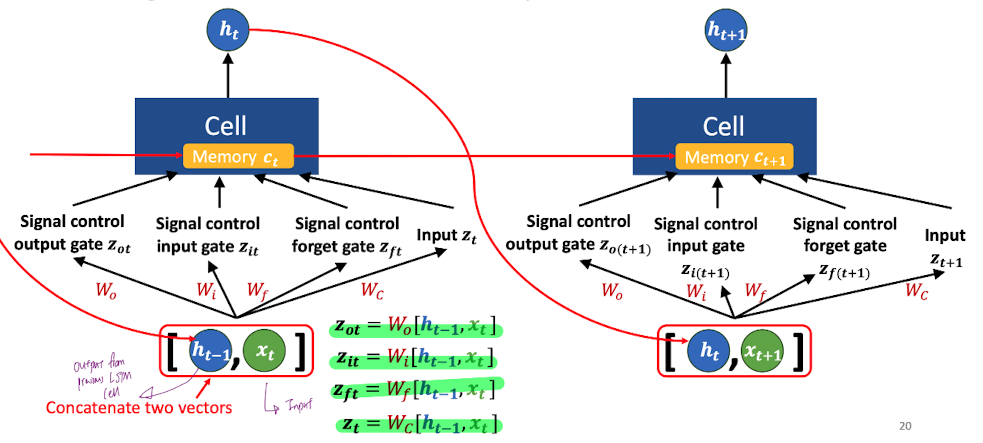
\includegraphics[width=0.95\linewidth]{27_lstm.png}
          \end{itemize}
          \item \textbf{Types of RNN:} (1): One-to-many (Image captioning), (2): Many-to-one (Sentiment analysis), (3): Many-to-many (Video classification with a label for each frame), (4): Encoder-decoder (Language Translation)
        \end{itemize}

        \subsection{Self-attention}
        \begin{itemize}
          \item \textbf{Motivation:} Unlike RNN which needs to wait for previous time steps, Self-attention model can capture context information without waiting for previous time steps
          \item \textbf{Procedure:} To calculate $h_i$
          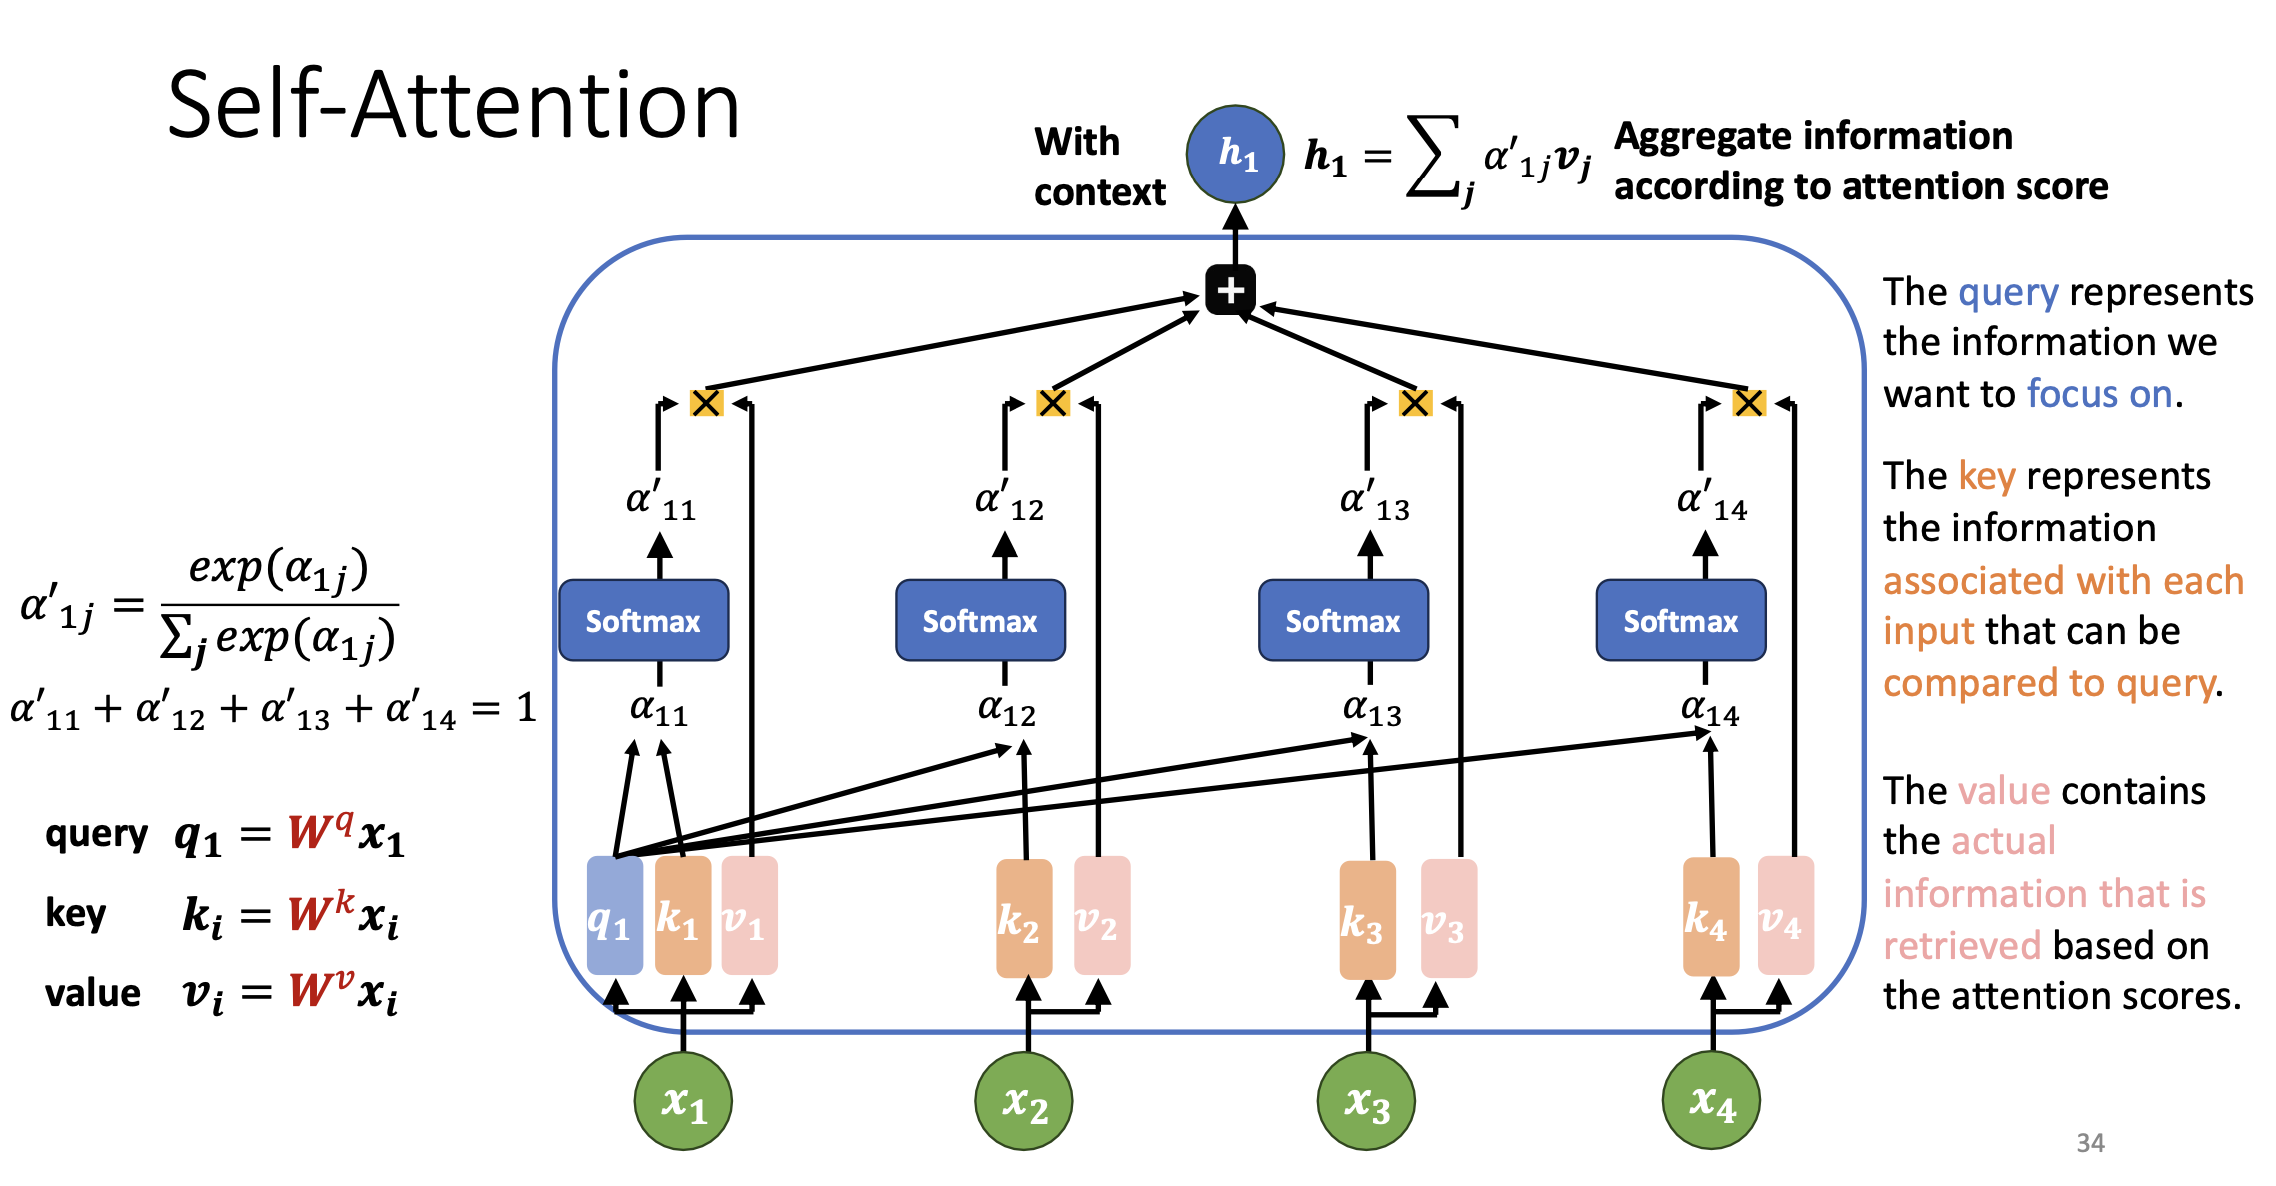
\includegraphics[width=0.95\linewidth]{28_self_attention.png}
          \begin{enumerate}
            \item Multiply $q_i$ (i = 1 in this case) with all $k_i$ → Obtain $\alpha_{ij}$
            \item Apply soft-max function to all $\alpha_{ij}$ and multiply resulting $\alpha'_{ij}$ with $v_j$
            \item Sum up all $\alpha'_{ij}v_j$ to obtain $h_i$
            \item Repeat 1-3 to obtain other $h_i$ values
          \end{enumerate}
        \end{itemize}

        \subsection{Issues with Deep Learning}
        \begin{enumerate}
          \item \textbf{Overfitting:} Addressed by dropout (randomly set some activations to 0 during neural network training, not the weights), early stopping (so that $J_{val}(w)$ does not increase)
          \item \textbf{Vanishing/Exploding Gradient:} Vanishing (small gradients multiplied again and again until it reaches almost 0), Exploding (Large gradients multiplied again and again until it overflows) $\rightarrow$ Addressed by non-saturating activation functions (ReLU) or Gradient Clipping (clip gradient within $[min, max]$)
        \end{enumerate}

        \section{Unsupervised Learning}
        \subsection{Supervised Learning VS Unsupervised Learning}
        \begin{itemize}
          \item \textbf{Supervised Learning:} Given a set of $m$ input-output pairs (training samples), learn to make a prediction
          \item \textbf{Unsupervised Learning:} Learning happens by experiencing data $\rightarrow$ Given a set of $m$ data points, learn patterns in data
        \end{itemize}

        \subsection{K-means Clustering}
        \begin{itemize}
          \item \textbf{Centroid:} Let points $x^{(i)}$ for $i=1,...,m_1$ be assigned to cluster 1 → For these points, Cluster Centroid is $\mu_1 = \frac{1}{m_1}\sum_{i=1}^{m_1}x^{(i)}$ ( $\mu_1, x^{(i)}$ are vectors)
          \item \textbf{K-means Algorithm (m data points, K centroids):}
          \begin{enumerate}
            \item Randomly initialise $K$ centroids $\mu_1,...,\mu_K$
            \item Repeat until convergence:
            \begin{itemize}
              \item For $i=1,...,m$: $c^{(i)} \leftarrow$ Index of cluster centroid $(\mu_1,...,\mu_K)$ closest to $x^{(i)}$ (Assign data points to centroid)
              \item For $k=1,...,K:$ $\mu_k \leftarrow$ Centroid of data points $x^{(i)}$ assigned to cluster $k$ (Reposition centroid based on data points)
            \end{itemize}
            \item No more changes in centroid positions $\rightarrow$ Converged (Can be shown that each step in algorithm never increases loss function)
          \end{enumerate}
          \item \textbf{Local Optima:} Possible for K-means to reach a local optimum where centroids do not move anymore, but loss might be high
          \item \textbf{K-means Loss Function:} Average distance of each sample to its centroid
          \item \textbf{K-Medoids:} Pick $K$ initial centroids randomly from points in data $\rightarrow$ Pick data points that is closest to centroids \& use them as centroids
          \item \textbf{Notes about K-means:}
          \begin{enumerate}
            \item Centroids are usually not located at 1 of the data points
            \item K parameter is chosen by the user
            \item Multiple restarts of the K-means give different solutions
          \end{enumerate}
        \end{itemize}

        \subsection{Hierarchical Clustering}
        \begin{itemize}
          \item \textbf{Purpose:} In a situation where we cannot decide on a fixed number of clusters, we want a hierarchy of clusters
          \item \textbf{Algorithm:}
          \begin{enumerate}
            \item Every data point is in a cluster
            \item Loop (until all points are in 1 cluster): Find a pair of cluster that “is nearest”, merge them together (NOTE: We have $N=2^n$ data points → Hierarchical Clustering algorithm produces a sequence of clusterings → Number of clusters in sequence is $N, N-1, ..., 1$ (Basically merge 2 clusters at 1 single time only))
          \end{enumerate}
          \item \textbf{Variants (Pick the minimum)}
          \begin{enumerate}
            \item \underline{Single Linkage:} Distance between closest elements in 2 clusters
            \item \underline{Complete Linkage:} Distance between furthest elements in 2 clusters
            \item \underline{Average Linkage:} Average of distances of all pairs in 2 clusters
            \item \underline{Centroid Method:} Distance between centroids of 2 clusters
          \end{enumerate}
          \item \textbf{Analysis:} It does not require number of clusters to be pre-defined, handles noise well, works well with non-linearly separable data, can be computationally expensive for large data sets ($O(n^3)$ to merge every cluster, where $O(n^2)$ to calculate distance for every pair \& $O(n)$ to find nearest pair) 
        \end{itemize}

        \subsection{Dimensionality Reduction}
        \begin{itemize}
          \item \textbf{Overview:} Many ML problems have data with high dimensional features → Number of samples to learn a hypothesis class increases exponentially with the number of features
          \begin{enumerate}
            \item \underline{Reduction:} Change basis of vector remove dependence between components, Remove non-important components that do not cause variations in data
            \item \underline{Reconstruction:} Add non-important components back, Restore basis
          \end{enumerate}
          \item \textbf{Singular Value Decomposition (SVD):} Take without loss of generality $n > m$, for any $n \times m$ rectangular real-valued matrix $X$, there exists a factorisation $X = U\sum V^T$
          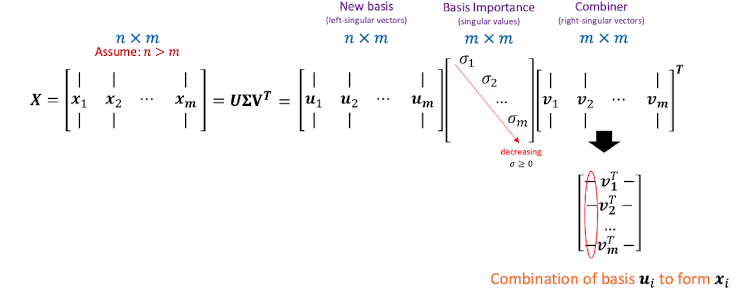
\includegraphics[width=0.95\linewidth]{29_SVD.png}
          \begin{enumerate}
            \item $U$ is $n \times m$ and has $m$ orthonormal columns
            \item $\sum$ is $m \times m$ and is diagonal with $\sigma_j \geq 0$ ordered from largest to smallest
            \item $V$ is $m \times m$ and has $m$ orthonormal columns and rows
          \end{enumerate}
          \item \textbf{Dimensionality Reduction via SVD:} Instead of $m$ singular values, we set all singular values except the first $r$ to 0 → Resulting matrix is the “best” approximation with new basis size of $r$ to the original matrix \\ Transforms from $n \times m = n \times m, m \times m, m \times m$ to $n \times m = n \times r, r \times r, r \times m$, where $r < m$
          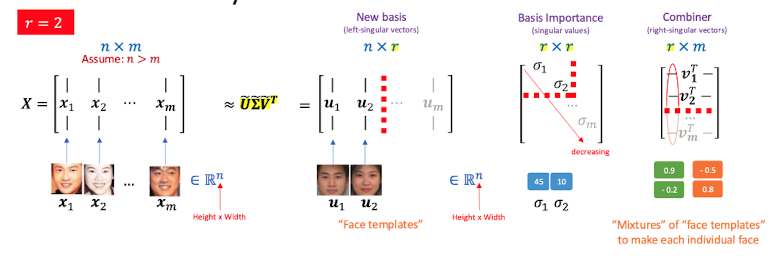
\includegraphics[width=0.95\linewidth]{30_dim_red_svd.png}
          \item \textbf{Reduction \& Reconstruction via SVD:} 
          \begin{enumerate}
            \item \underline{Data Matrix ($n \times m$):} $X = U \sum V^T \approx \tilde{U}\tilde{\sum}\tilde{V}^T$
            \item \underline{Reduced Data ($r \times m$):} $Z = \tilde{U}^TX$
            \item \underline{Reconstructed Data ($n \times m$):} $\tilde{X} = \tilde{U}Z$
          \end{enumerate}
          \item \textbf{r-SVD}: defines an encoder-decoder structure for reduction and reconstruction of high-dimensional data
          \item \textbf{Principal Component Analysis (PCA):} Captures components that max the statistical variations of the data
          \begin{enumerate}
            \item Given the data matrix $X=(x^{(1)},...,x^{(m)})$, where $x^{(i)}$ is the $i^{th}$ row of $X$
            \item Compute mean over samples: $\overline{x} = \frac{1}{m}\sum_{i=1}^m x^{(i)}$
            \item Compute mean-centred data: $\hat{x}^{(i)}= x^{(i)} - \overline{x}$
            \item Define data matrix $\widehat{X}=(\hat{x}^{(1)},...,\hat{x}^{(m)})$
            \item Create covariance matrix of data: $Cov(X)= \frac{1}{m}\widehat{X}\widehat{X}^T$
            \item Compute SVD on $Cov(X)$ to obtain the $U$ matrix
            \item Reduce to $r$ components to obtain $\widetilde{U}$ (choose minimum $r$ s.t. $\frac{\sum_{i=1}^r \sigma_i^2}{\sum_{i=1}^m \sigma_i^2} \geq 0.99$, where at least 99\% of variance in data is retained)
          \end{enumerate}
        \end{itemize}
  \end{multicols*}
  \hrulefill
% \\\begin{multicols}{3}
%   \subsection{Entropy Table}
%     $I(\frac{row}{row+col}, \frac{col}{row+col})$
%     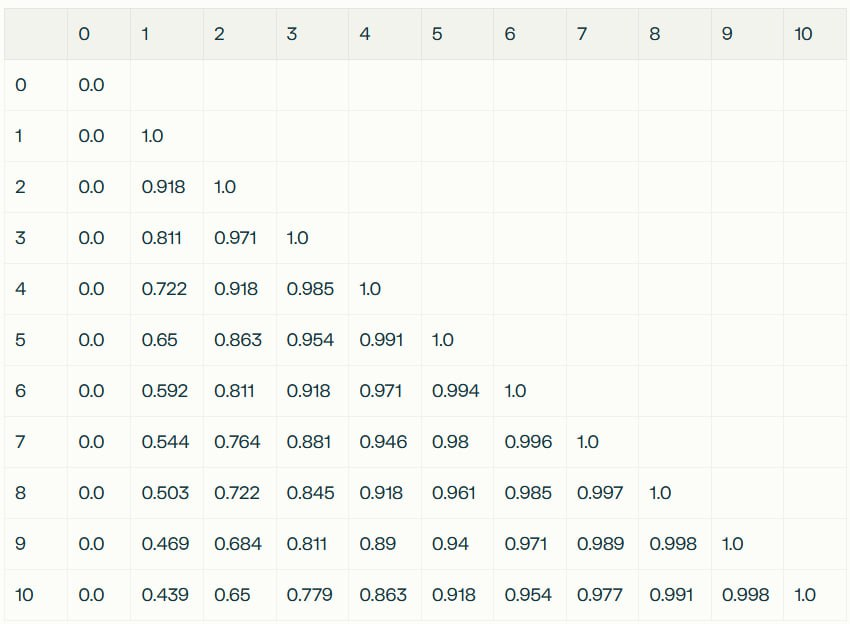
\includegraphics[width=0.95\linewidth]{14_entropy_table.jpg}
%   \end{multicols}
%   \hrulefill
% \\\begin{multicols}{1}
%     \subsection{Log Base 2 Table}
%       $log(\frac{col}{row})$
%       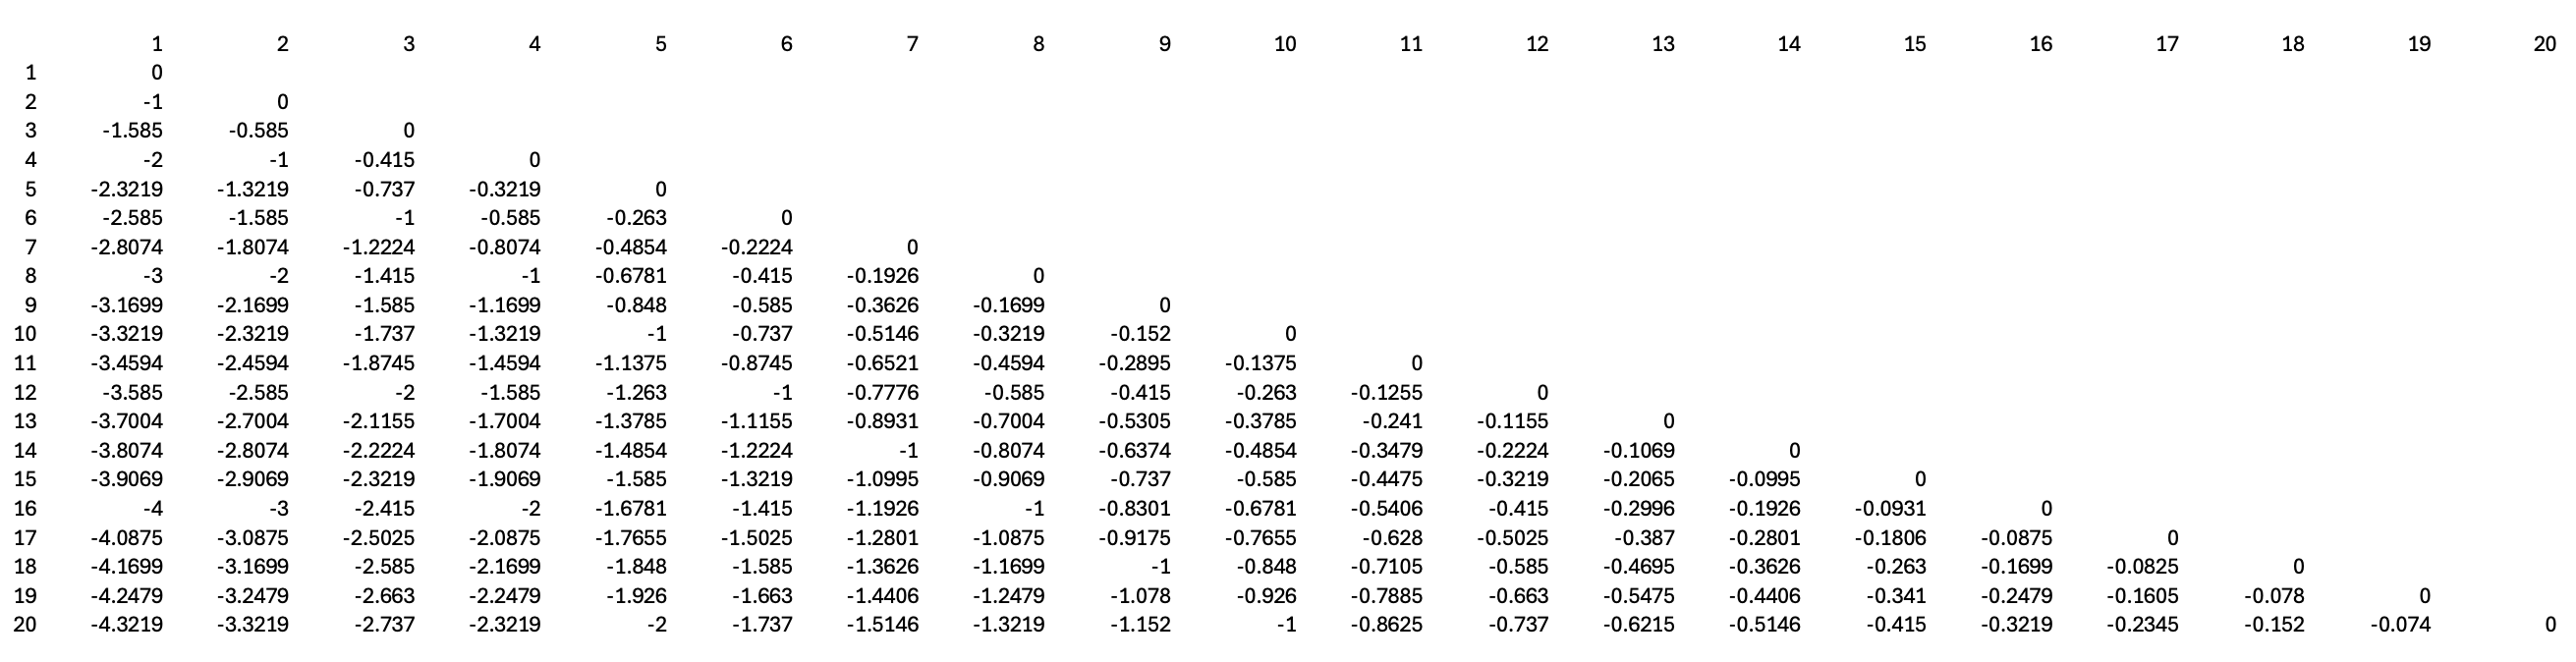
\includegraphics[width=1.5\linewidth]{15_log_base_two.png}
%   \end{multicols}
\end{document}
